%% main.tex 2025/04/04
%
% Based on sample files of unknown authorship.
%
% The Current Maintainer of this work is ICT Department @ ENIT.
% National Engineering School of Tunis. https://enit.rnu.tn/
% Information and Communication Technologies Department

\documentclass[a4paper,12pt, final]{report}
\usepackage[utf8]{inputenc}
\usepackage[T1]{fontenc}
\usepackage[english]{babel}
\usepackage{acronym}
\usepackage{algorithm}
\usepackage{algorithmic}
\usepackage{amsfonts}
\usepackage{amsmath}
\usepackage{amssymb}
\usepackage{array}
\usepackage{booktabs}
\usepackage{comment}
\usepackage{caption}
\usepackage{subcaption}
\usepackage{dirtytalk}
\usepackage{enumitem}
\usepackage{tikz}
\usepackage{fancyhdr}
\usepackage{float}
\usepackage{geometry}
\usepackage{graphicx}
\usepackage{indentfirst}
\usepackage{lmodern}
\usepackage{longtable}
\usepackage{makecell}
\usepackage{mathrsfs}
\usepackage{microtype}
\usepackage[nottoc]{tocbibind}
\usepackage{siunitx}
\usepackage{textpos}
\usepackage{titlesec}
\usepackage{url}
\usetikzlibrary{positioning, fit, calc, arrows.meta, shapes.geometric}
\usepackage[pages=some]{background}
%\captionsetup[table]{position=bottom}
\numberwithin{equation}{section}

%pagestyle
\pagestyle{fancy}
\fancyhf{}
\cfoot{\thepage}
\newcommand{\euro}{\EUR\xspace}

\begin{document}
\backgroundsetup{
scale=1,
color=black,
opacity=1,
angle=0,
contents={%
  
\includegraphics[width=19cm,height=28.5cm]{figures/background.png}
  }%
}
\begin{titlepage}
\BgThispage
\begin{textblock}{1.5}[0.5,0.5](0.5,0.5)
	
\includegraphics[width=\linewidth]{figures/logoUTM.png}\\[3.5cm]
  \end{textblock}
  
\begin{textblock}{2}[0.5,0.5](9.7,0.15)
	
\includegraphics[width=\linewidth]{figures/logoEnit.png}\\[2cm]
  \end{textblock}

\begin{center}
{University of Tunis El Manar\\[0.2cm]
\textbf{National Engineering School of Tunis}\\[0.2cm]
Information and Communication Technologies Department}\\[1cm]
{\Large \textbf{Final Year Project Report}}\\[0.6cm]

{\emph{Submitted by:}}\\[0.3cm]
{\large \textbf{Mootez KNISS}}\\
\vspace{0.5cm}
{\emph{In partial fulfillment of the requirements for the: }}\\[0.3cm]
%{\large \textbf{National Engineering Degree in Computer Science}}
{\large \textbf{National Engineering Degree in Telecommunications}}

% Title
\rule{\linewidth}{0.5mm} \\[0.1cm]
{ \huge \bfseries Smartcare Usecase
 \\[0.1cm] }
\rule{\linewidth}{0.5mm} \\[0.5cm]

% Host Company
{\emph{Host Company:}}\\
{\textbf{Huawei}}\\
%
\includegraphics[width=2cm]{figures/company_logo.png} \\[2cm]
\end{center}

% Date
\noindent
{\emph{Defense Date:}} {\textbf{date}}\\

%Jury Members 
\begin{table}[H]
\begin{tabular}{ll}

\emph{Jury Members:} \vspace{0.7cm} & \\
President: & \begin{tabular}[c]{@{}l@{}}\textbf{Mrs Sonia DJAZIRI LARBI} \end{tabular} \\
Reviewer: & \begin{tabular}[c]{@{}l@{}}\textbf{Mrs. Asma BEN HAMED}  \end{tabular}\\
Company Supervisor: & \begin{tabular}[c]{@{}l@{}}\textbf{Mrs. Manel MAAMER}  \end{tabular}\\
ENIT Supervisor: & \begin{tabular}[c]{@{}l@{}}\textbf{Mr. Taher EZZEDINE}  \end{tabular}

\end{tabular}
\end{table} 


\vspace{1.5cm}
% Bottom of the page
\centering{Academic Year: 2025-2026}

\end{titlepage}
\thispagestyle{empty}
\newpage
\thispagestyle{empty}
\newpage
\newpage
\section*{Dedication}

%%%%%% NB. It is more personal compared to the acknowledgments.

\vspace{1cm}
\par \textbf{I} would like to dedicate my end-of-studies project to all the
friends and family who stood by me through my lowest moments and my highest:
my mother and my siblings, with special thanks to my sister May for helping me
whenever I asked; and my father, may Allah have mercy on him, for always pushing
me, even from beyond the grave.

I hope this project will be just the first of many to make you all proud.

\newpage
\section*{Acknowledgments}

\vspace{1cm}

\par \textbf{F}irst and foremost, I thank \textbf{Allah Almighty} for granting
me the health, the patience and the ability to see this project through to the
end.

I would like to express my sincere gratitude to my ENIT supervisor,
\textbf{Mr. Taher EZZEDINE}, for his guidance and his feedback throughout this
project.

My thanks go equally to my company supervisor at Huawei,
\textbf{Mrs. Manel MAAMER}, for her availability, her advice, and for giving me
the freedom to take this project in the direction it needed to go.

I also wish to thank the \textbf{Sales and Solutions Department at Huawei}, and
in particular the colleagues who took the time to answer my questions about
SmartCare and who helped me find my footing in a domain that was new to me.

I would like to thank the \textbf{members of the jury} for taking the time to
read and evaluate this work.

Finally, my deepest thanks go to my \textbf{family} and my \textbf{friends}, for
their patience and their constant encouragement throughout my studies. None of
this would have been possible without them.

\chapter*{Abstract}

\par Write your English abstract here


{\large \textbf{Keywords} : }Natural language processing, Artificial intelligence, Keyword, Keyword

\newpage
\section*{Résumé}
 Résumé en français ... \\
 \textbf{Mots clés} : Traitement Automatique du Langage Naturel, Intelligence Artificielle, Mot clé, Mot clé



\thispagestyle{empty}
\newpage

\vspace{2\baselineskip}

\tableofcontents
\thispagestyle{empty}

\listoffigures
\listoftables
\thispagestyle{empty}
\newpage
\chapter*{List of Acronyms}
\addcontentsline{toc}{chapter}{List of Acronyms}

%%%%%% NB. Please ensure that the acronym list is maintained in alphabetical order.

\vspace{1cm}
\begin{itemize}
    \item \textbf{AI:} Artificial Intelligence.
    \item \textbf{API:} Application Programming Interface.
    \item \textbf{ARPU:} Average Revenue Per User.
    \item \textbf{AWS:} Amazon Web Services.
    \item \textbf{BM25:} Best Matching 25, a lexical ranking function used in retrieval.
    \item \textbf{BSS:} Business Support System.
    \item \textbf{CPU:} Central Processing Unit.
    \item \textbf{CSV:} Comma-Separated Values.
    \item \textbf{FAISS:} Facebook AI Similarity Search, a vector similarity library.
    \item \textbf{FWA:} Fixed Wireless Access.
    \item \textbf{GPU:} Graphics Processing Unit.
    \item \textbf{HTML:} HyperText Markup Language.
    \item \textbf{HVC:} High-Value Customer.
    \item \textbf{JSON:} JavaScript Object Notation.
    \item \textbf{KPI:} Key Performance Indicator.
    \item \textbf{LLM:} Large Language Model.
    \item \textbf{LTE:} Long-Term Evolution.
    \item \textbf{MBB:} Mobile Broadband.
    \item \textbf{MQTT:} Message Queuing Telemetry Transport.
    \item \textbf{MSISDN:} Mobile Station International Subscriber Directory Number, the
    subscriber's phone number, used here as the key joining the two databases.
    \item \textbf{NPS:} Net Promoter Score.
    \item \textbf{ODA:} Open Digital Architecture, TM Forum's reference architecture.
    \item \textbf{OSS:} Operations Support System.
    \item \textbf{QoE:} Quality of Experience.
    \item \textbf{RAG:} Retrieval-Augmented Generation.
    \item \textbf{ReAct:} Reason and Act, an agent pattern interleaving reasoning steps
    with concrete actions.
    \item \textbf{RSRP:} Reference Signal Received Power.
    \item \textbf{SINR:} Signal-to-Interference-plus-Noise Ratio.
    \item \textbf{SMOTE:} Synthetic Minority Over-sampling Technique.
    \item \textbf{SMS:} Short Message Service.
    \item \textbf{SQL:} Structured Query Language.
    \item \textbf{TCA:} Threshold-Crossing Alert.
    \item \textbf{TM Forum:} TeleManagement Forum, the industry body whose data models
    the schema in this project is based on.
    \item \textbf{UI:} User Interface.
    \item \textbf{VoLTE:} Voice over LTE.
    \item \textbf{VRAM:} Video Random Access Memory.
    \item \textbf{XGBoost:} Extreme Gradient Boosting.
\end{itemize}


%%%%%%%%%%%%%%%%%%%%%%%%%%%%%%%%%%%%%%%%%%%%%%%%
%%%%%%%%%%%%%%%%%%%%%%%%%%%%%%%%%%%%%%%%%%%%%%%%

\chapter*{General introduction}
\addcontentsline{toc}{chapter}{General introduction}
Artificial Intelligence has advanced to a point where failing to leverage it — even at its most basic — risks falling behind. The time saved through AI and LLMs is too valuable to ignore, allowing research \& development to be further accelerated, but also complex data-driven operations — where decisions once required teams of analysts and hours of querying — to be handled in seconds through natural conversation. This applies especially in the telecommunications field, where the industry is too data sensitive, as it generates a vast amount of network performance metrics, subscriber behavior data and commercial indicators in real time. Usually this process is done through dedicated teams, specialized tools and significant time investment. However with the emergence of LLMs and their advanced reasoning, as well as agentic AI, it is now possible for one operator to simply ask a question and receive a well informed, data-backed response promptly. The project explores this possibility further, building an AI-powered network analytics assistant that allows network operators to query, analyze and act on both network and commercial data through natural language alone in order to help improve customer experience and boost revenue.

Today, a commercial manager who would want to identify upsell opportunities in a specific region, for instance 5G upsell, and how to approach this upsell campaign, would need to file a request to a data analyst in order to consult strategies and best in slot options. Accessing the data is rarely the bottleneck. Modern telecom operators have dashboards, BI tools, etc... The real issue is what comes after extracting said data, yes it would take time to get the right query in order to get exactly what the manager wants, but what takes even more time is making sense of it: raw metrics in isolation mean little; their value emerges only when contextualized/correlated, and interpreted across multiple dimensions simultaneously. A single anomaly in network performance could be insignificant on its own, might even just be an outlier — but viewed alongside subscriber complaint patterns, billing trends and geographic coverage gaps, that same anomaly can turn out to be the first sign of something worth acting on. Arriving at the right conclusion requires not just data access, but cross-domain expertise, time and collaborative analysis across multiple teams.

Stated formally: given a telecom operator's OSS and BSS databases $D_{net}$ and $D_{com}$, and a natural-language question $q$ posed by a non-technical user, the problem is to produce an answer $A(q)$ that is correct with respect to the current state of those databases, delivered in interactive time, and where any action with operational consequence is proposed for human approval rather than executed autonomously.

In response to this challenge, this project sets out to develop an AI-powered conversational assistant for telecom operators, capable of running queries quickly, and more importantly, correctly analyze and come up with solutions/suggestions/overview, reducing dependency on technical teams for day-to-day analytical tasks.
The specific objectives, each stated with the criterion used to judge it:
\begin{itemize}
    \item \textbf{A representative simulated environment.} Two databases split along
    the OSS/BSS line, schema derived from TM~Forum's Information Framework, populated
    with $\sim$50{,}000 internally consistent subscribers and joinable on a single key.
    \item \textbf{Multi-step natural-language reasoning across both domains.} The agent
    chains more than one query when a single one cannot answer the question, and
    inspects the real schema rather than guessing column names. Target: at least 80\%
    correct on a golden set of factual questions with independently computed answers.
    \item \textbf{Responses grounded in domain knowledge.} Every query is written
    against the live schema through a knowledge graph and retrieval over worked
    examples; answers citing numbers absent from the query results are rejected and
    regenerated automatically.
    \item \textbf{Operations beyond answering.} Charts, an interactive drill-down mind
    map, a segment-to-strategy diagram, and CSV export available on eligible answers.
    \item \textbf{A continuously live environment.} A simulator advances both databases
    on a fixed tick rather than regenerating on demand, so no answer can be reused
    without re-querying. Target: no data series more than one reporting cycle stale.
    \item \textbf{Human approval for operational actions.} Every action with external
    consequence is proposed, never executed. Target: zero autonomous executions on
    adversarial prompts.
\end{itemize}

Chapter~\ref{ch:eval} reports the measured outcome against each of these criteria,
including the ones that were not met.

\subsection*{Contributions}

The specific contributions of this work are:
\begin{enumerate}
    \item A dual-database synthetic telecom environment with a \emph{causally coupled}
    simulator, in which a raised fault degrades its own cell's counters, propagates to
    the customers that cell serves, and raises their churn risk until it heals ---
    rather than each of those being an independent random process.
    \item An agent architecture that combines structured tool-calling with
    schema-graph retrieval and a deterministic post-hoc verification layer, so that
    factual correctness is enforced by code rather than requested in a prompt.
    \item A disambiguation mechanism that declines to answer an under-specified
    question, offering concrete readings of it instead of silently choosing one.
    \item A human-in-the-loop action pipeline in which the agent may propose an
    operational action but never execute it.
    \item An empirical observation that the failure modes of this system persist
    across a substantial increase in model size, locating the remaining errors in the
    retrieval and grounding layer rather than in model capacity --- with a measured
    evaluation, including failures, reported rather than omitted.
\end{enumerate}


The project follows an empirical, iterative methodology — driven by experimentation and progressive refinement rather than a predefined specification. Approaches were selected, tested, and either validated or discarded based on observed results, making the development process as much a research exercise as an engineering one.

As a result, the scope was redefined to what is feasible rather than what was initially planned; it is now bounded to a simulated telecom environment representing a hypothetical operator with around 50{,}000 subscribers across a fictional geography, covering the network domain in sites, cells, KPIs and alarms, as well as the commercial domain via subscribers, billing, churn and campaigns. Real-time hardware integration, production infrastructure, and multi-operator scenarios fall outside the current scope for now.

The produced deliverables are:
\begin{itemize}
    \item Dual database simulated telecom environment, with dynamic data simulator.
    \item A conversational AI agent capable of natural language querying and operational action execution such as excel export.
    \item A churn prediction model integrated into the live environment
    \item Real time dashboard surfacing network and commercial intelligence
    \item A RAG knowledge base grounding the agent in telecom domain
\end{itemize}

The rest of this report follows the order the work actually happened, rather than
a tidy after-the-fact architecture.

\textbf{Chapter~\ref{ch:context}} covers the host organization and the context the
project sits in --- what SmartCare is, and why building against it directly was
never an option.

\textbf{Chapter~\ref{ch:related}} positions the work against existing research in
text-to-SQL, language-model agents, and retrieval-based grounding, and is explicit
about which parts of the design are established technique and which are not.

\textbf{Chapter~\ref{chapter:BF-DFP}} lays the foundation: two synthetic databases
modelled on TM Forum's abstractions, a first agent loop running on a local model
to prove the idea works, and then the move to cloud inference once local hardware
turned out to be the ceiling rather than the idea itself.

\textbf{Chapter~\ref{ch:livingdb}} turns that static data into a living environment
--- a simulator that keeps KPIs, alarms, incidents and churn moving, so the
assistant is always reading a target that never sits still.

\textbf{Chapter~\ref{ch:agent}} covers the agent itself: the reasoning loop, how it
grounds its queries in the real schema instead of guessing, how it catches its own
mistakes before they reach the user, and everything it can do beyond answering in
plain text.

\textbf{Chapter~\ref{ch:eval}} measures all of it against a golden set, reports
where it fails, and documents a churn model that was found not to transfer.

\textbf{Chapter~\ref{ch:limits}} sets out what the system does not do, what that
costs, and what would have to happen next.


\chapter{Host Organization and Project Context}\label{ch:context}
\section*{Introduction}
Before diving into the technical work, it is important to understand the environment in which it was carried out --- who the host organization is, what they do, and why this project exists in the first place. This chapter covers exactly that. We start with an overview of Huawei as a company: its history, mission, and how it is structured internally. We then zoom into the Sales and Solutions Department, which hosted this internship, and the SmartCare platform that sits at the core of the project. From there, we shift to the project context itself --- the industry background, the technological factors at play, and the specific challenges that motivated the work. By the end of this chapter, the problem this project is solving 
should be clear, and the rest of the report can be read with that foundation in mind.

\section{Host Organization: Huawei}
\begin{figure}[htbp]
    \centering
    
\includegraphics[width=0.2\textwidth]{figures/company_logo.png}
    \caption{Company Logo}
    \label{fig:company-logo}
\end{figure}

\subsection{Company Overview}
Founded in 1987 in Shenzhen, China, Huawei Technologies Co., Ltd. is a leading global 
provider of Information and Communications Technology (ICT) infrastructure and smart 
devices. With approximately 213,000 employees operating across more than 170 countries 
and regions, Huawei serves upwards of 3 billion people worldwide \cite{huawei_about}. 
Over nearly four decades, the company has evolved from a sales agent for Private Branch 
Exchange (PBX) switches into one of the world's largest technology corporations, 
sustaining this growth through a sustained commitment to research and development: in 
2025 alone, Huawei invested CNY~192.3 billion in R\&D, representing 21.8\% of its total 
revenue, with over 53\% of its workforce engaged in research activities \cite{huawei_about}.

Within its carrier-facing portfolio, Huawei offers a broad range of solutions to help 
Communication Service Providers (CSPs) operate and optimize their networks --- and among 
those, \textbf{HUAWEI SmartCare} is one of the flagship ones. To keep it simple, 
SmartCare is a Customer Experience Management (CEM) platform: it brings together network 
analytics, subscriber management, and service assurance all in one place 
\cite{huawei_smartcare_cem}. It was originally built as a Service Operations Center (SOC) 
solution, the idea being to stop operators from always playing catch-up with network 
issues and instead get ahead of them --- detecting degradation before it reaches the end 
user \cite{huawei_smartcare_soc}.

At its core, SmartCare works through a three-tier indicator framework --- Customer 
Experience Indicators (CEIs), Key Quality Indicators (KQIs), and Key Performance 
Indicators (KPIs) --- giving operators a per-service, per-user, per-location view of what 
is actually happening on the network. It also covers QoE monitoring, fault
diagnosis, NPS tracking, and self-care integration. Gartner lists it as a
Representative Vendor for CSP service and network assurance, and it is certified
under the TM Forum ODA component directory
\cite{huawei_gartner}\cite{huawei_tmforum}.

This internship builds on that foundation with a new use case for the Sales and
Solutions Department: a conversational AI layer powered by a Large Language Model
(LLM), plus a churn prediction module. That was the brief at the start; what the
churn side actually became, and why, is covered in Chapter~\ref{ch:eval}. The
goal is to let sales and solutions engineers query live subscriber and network
data in plain language and surface at-risk subscribers --- extending SmartCare
into pre-sales and account management, where it currently doesn't reach.

\subsection{Mission and Strategic Vision}

Huawei's guiding mission is to bring digital to every person, home, and organization 
for a fully connected, intelligent world. This mission is operationalized through the 
company's All Intelligence Strategy, unveiled in 2023, which places AI at the center 
of every business domain --- from network infrastructure to enterprise cloud services 
to consumer devices.

The company's strategic pillars as articulated in its 2025 commitments are:
\begin{itemize}
    \item \textbf{Laying the groundwork for All Intelligence} --- building the 
    foundational infrastructure for an AI-driven era across industries.
    \item \textbf{Strengthening innovation, openness, and collaboration} --- investing 
    in basic research while remaining open to ecosystem partnerships.
    \item \textbf{Succeeding through quality and prioritizing security} --- treating 
    quality as a precondition for customer trust and long-term competitiveness.
    \item \textbf{Building thriving ecosystems for a shared future} --- fostering 
    developer communities (Kunpeng, Ascend, HarmonyOS) and partner networks.
    \item \textbf{Promoting sustainable development through digital inclusion} --- 
    extending connectivity to underserved populations and reducing carbon footprints 
    through digital power solutions.
\end{itemize}

Quality occupies a central place in Huawei's corporate culture, formalized in its 
Quality Policy: ``Always keep in mind that quality is the foundation of Huawei's 
survival, and the reason for the customer to choose Huawei.''

\subsection{Organizational Structure}

Huawei runs on a \textbf{matrix organizational model} --- product-line specialization 
on one axis, regional customer proximity on the other. The company is structured around 
three primary Business Groups (BGs) and two dedicated Business Units (BUs), as shown 
in Table~\ref{tab:huawei_org}.

\begin{table}[h!]
\centering
\renewcommand{\arraystretch}{1.4}
\begin{tabular}{|p{5.5cm}|p{8.5cm}|}
\hline
\textbf{Division} & \textbf{Focus Area} \\
\hline
Carrier Business Group (Carrier BG) & Wireless networks, fixed networks, core networks, 
carrier software, and global services for telecommunications operators \\
\hline
Enterprise Business Group (Enterprise BG) & Data center infrastructure, storage, and 
digital transformation solutions for enterprises and industries \\
\hline
Consumer Business Group (Consumer BG) & Smartphones, PCs, tablets, wearables, HarmonyOS 
ecosystem, and intelligent driving solutions \\
\hline
Cloud \& AI BU & Cloud computing services, AI platforms (Pangu Models), and developer 
ecosystems (Kunpeng, Ascend) \\
\hline
Digital Power BU & Energy-efficient power solutions, green energy generation, and smart 
grid infrastructure \\
\hline
\end{tabular}
\caption{Huawei Business Groups and Units}
\label{tab:huawei_org}
\end{table}

\subsection{Regional and Sales Structure}

On the commercial side, operations are split across geographic regions, each under a 
Regional Sales Vice President who oversees the country-level offices below them. Day 
to day, it's a dual-track setup: \textbf{lead account teams} at headquarters keep an 
eye on the big accounts, while \textbf{local channel teams} and regional enterprise 
teams handle the actual delivery, customization, and partner work on the ground. 
Global product capabilities, local execution --- that's the idea.

This internship was carried out within the \textbf{Sales and Solutions Department}, 
sitting under the Carrier Business Group. The department's job is essentially to 
translate Huawei's technical portfolio into something a customer can act on --- 
proposals, demos, data-driven recommendations. SmartCare is one of the core platforms 
they present and sell, which is exactly what made it the right home for this project.

\section{Project Context}

\subsection{Background}

\subsubsection{Historical Context}

In the telecom and operator industry, the past three decades have brought profound 
structural change. Networks evolved from Circuit-Switched (CS) voice in 2G, to 
Packet-Switched (PS) architectures in 3G, through Long-Term Evolution (LTE) in 4G, 
and up to the current deployment of fifth-generation (5G) networks. This progression 
not only improved bandwidth and latency, but gave rise to an unprecedented volume of 
operational data --- KPIs, KQIs, network campaigns, and subscriber behavior records 
accumulating at a scale that traditional tooling was never designed to handle. 
Network hardware vendors such as Huawe, which delivered the world's first commercial LTE/EPC network 
in 2009 and has since supported the deployment of 5G as well, across more than 170 countries 
worldwide, have gathered expertise in managing this complex, multi-layered infrastructures. Yet 
the tools used to query, interpret and act upon the data they produce have historically been the 
drawback, relying on dashboards, manual reporting and siloed analyst workflows. SmartCare was built to 
help close that gap on the network ops side, but the sales layer wasn't really touched.

However this changed after the emergence of LLMs between 2020 and the present, a new frontier has opened:
the ability to query structured operational data in plain natural language, without SQL expertise 
or intimate knowledge of database schemas. But beyond just fetching data, an LLM can reason over the results, 
spot patterns and give a conclusion, helping a sales manager or solutions engineer to get to the 
right question faster, without relying on a data analyst on standby.
\subsubsection{Socioeconomic and Technological Factors}

Several converging factors shaped the environment in which this project was conceived. 
The commercial rollout of 5G introduced a new layer of network complexity, with 
operators now managing simultaneous multi-generation subscriber bases spanning 2G 
through 5G --- each with distinct usage profiles, churn behaviors, and upgrade 
trajectories. Migrating subscribers toward newer technologies therefore requires a 
strategic viewpoint and surgical precision when analyzing network variables, making 
data-driven tooling not just convenient but operationally necessary.

On the infrastructure side, while LLMs are inherently resource-intensive, a company 
of Huawei's scale can leverage cloud-hosted inference APIs, ensuring access to the 
latest high-reasoning models without the overhead of local hardware provisioning. 
That said, data privacy regulations and enterprise security requirements impose 
constraints on what data can be externalized to commercial services --- reinforcing 
the need for locally deployable or tightly controlled inference solutions as a 
complementary approach.

\subsubsection{Current Challenges}\label{sec:challenges}

Despite the availability of rich operational data --- and despite SmartCare already 
handling the network operations side --- several challenges persist when it comes to 
actually using that data in a sales and solutions context. Database schemas in 
telecom environments are large, relational, and non-trivial: even experienced 
analysts make errors constructing queries across multi-table subscriber and network 
datasets. Churn prediction, something carrier customers care a lot about, typically 
requires a purpose-built machine learning pipeline --- and those are rarely integrated 
with the conversational or dashboard tools sales teams actually use. On top of that, 
the time between a business question coming up in a customer meeting and getting a 
data-backed answer is still too long, which limits how agile a solutions engagement 
can be.

These gaps --- raw data vs.\ actionable insight, ML outputs vs.\ operational 
dashboards, natural language questions vs.\ structured query results --- are exactly 
what this project is trying to close, by bringing that capability into SmartCare's 
ecosystem.

\bigskip
\noindent The following section defines the specific problem statement this project 
was designed to solve, drawing directly from the operational context described above.
\section{Conclusion}
In this chapter, we introduced Huawei as the host organization --- its history, structure, and the SmartCare platform that sits at the center of this project. We also laid out the context that motivated the work: a telecom industry generating more operational data than existing tools can handle, and a sales layer that still largely relies on manual effort to make sense of it. The following chapters get into the actual work --- starting with the system architecture and the data foundation we built to support it.

\chapter{State of the Art and Related Work}\label{ch:related}

\section*{Introduction}
\addcontentsline{toc}{section}{Introduction}

Asking a database a question in plain language is not a new idea, and neither is
wrapping a language model in a loop so it can go and do things. What is a lot
less settled is what happens when you put those two ideas together on top of
operational data that keeps changing while you are querying it, and when the
answers coming out are meant to drive commercial decisions about real customers.
So where does this project actually sit? This chapter places the work against
the research it borrows from, and is upfront about which parts are established
technique and which parts are ours.

\section{From Semantic Parsing to Text-to-SQL}

The systems discussed throughout this chapter rest on the transformer
architecture\cite{Attention} and on the observation that sufficiently large
language models can perform tasks from a handful of in-context examples rather
than task-specific training\cite{gpt3}, later sharpened by tuning models to
follow instructions directly\cite{instructgpt}.

Translating natural language into database queries has been studied for decades,
but the modern framing dates to two benchmark datasets. WikiSQL~\cite{seq2sql}
paired natural-language questions with SQL over single tables, and demonstrated
that sequence-to-sequence models could learn the mapping directly.
Spider~\cite{spider} raised the difficulty substantially by requiring queries
that span multiple joined tables across databases the model has never seen, which
made schema generalisation --- rather than sentence parsing --- the central
problem.

That shift matters a lot for this project. A system that memorises the mapping
from question phrasing to query template becomes useless the moment the schema
changes, and our environment changes continuously. The response in the research
has been to hand the model the schema as context rather than baking it in as
training data.
General-purpose language models proved surprisingly capable at this without
task-specific training~\cite{llm_text2sql_eval}, and systematic benchmarking has
since mapped how prompt design, schema representation and example selection each
move accuracy~\cite{dailsql}.
DIN-SQL~\cite{dinsql} decomposes a hard question into simpler sub-problems and
adds a self-correction pass, reporting that decomposition plus correction
outperforms asking for the whole query in one shot.

Our agent follows that same principle without taking the method wholesale: it
decomposes by taking one action at a time inside a loop rather than asking the
model to plan out sub-queries, and its self-correction is a deterministic check
against the real schema instead of another model call. The reasoning is
something this report comes back to again and again --- a check the model
performs is a check the model can decide to skip.

\section{Language-Model Agents and Tool Use}

Chain-of-thought prompting~\cite{cot} established that eliciting intermediate
reasoning improves performance on multi-step problems, but reasoning alone
cannot consult a database. ReAct~\cite{react} closed that gap by interleaving
reasoning steps with concrete actions against an external environment and
feeding the observations back, which is precisely the cycle at the centre of
Chapter~\ref{ch:agent}. Later work extended the pattern in two directions: searching over several
candidate reasoning paths rather than committing to one~\cite{tot}, and having an
agent critique its own previous attempt before retrying~\cite{reflexion}. Both are
relevant to a loop that must recover from a query returning nothing.
Toolformer~\cite{toolformer} approached the same problem
from the other direction, training a model to decide for itself when to call an
external tool.

We use the ReAct pattern here with one significant practical difference. In the
original version the model writes its action as text and the surrounding program
parses it back out. Our first prototype did exactly that, and hit the predictable
failure: nothing actually forces the model to respect that format, and a small
drift in phrasing breaks the parse silently. Swapping that convention for a
provider-validated tool-calling interface wiped out an entire class of failure
without changing the loop at all --- which is a point about engineering rather
than agent design, but it is the thing that decided whether the system worked.

\section{Retrieval and Grounding}

Retrieval-augmented generation~\cite{rag} established the general remedy for a
model reasoning about knowledge it does not have: retrieve the relevant material
and place it in context rather than relying on parameters. The technique is
normally applied to document collections; here it is applied to schema and query
knowledge, retrieving the subgraph of tables and join paths relevant to a
question along with worked SQL examples.

Retrieval quality rests on established components. BM25~\cite{bm25} provides
lexical matching, which matters when a question names a column almost exactly,
and dense retrieval provides the semantic half~\cite{dpr}, implemented here over
sentence embeddings~\cite{sbert} indexed with FAISS~\cite{faiss} --- which matters
when the question does not name the column at all. Combining both is standard practice, and this system does so.

Where we depart from the retrieval literature is in what happens after
generation. Retrieval lowers the chance of an ungrounded answer, but it does not
detect one, and the tendency of these systems to produce fluent unsupported
content is well documented\cite{hallucination_survey}. The verification layer in Chapter~\ref{ch:agent} --- checking that
every cited number appears in the retrieved rows, and that every claim of absence
has a query behind it --- is a post-hoc deterministic check rather than a
retrieval improvement, and Chapter~\ref{ch:eval} shows both that it catches real
failures and that it misses an entire class of them.

\section{Telecom Analytics and Customer Experience Management}

The operational context is described by the TM~Forum Information
Framework~\cite{tmforum_sid}, which defines the data domains an operator
manages and the OSS/BSS separation the database design in
Chapter~\ref{chapter:BF-DFP} mirrors. Commercial customer-experience platforms,
including the SmartCare product this project was undertaken alongside, operate
over exactly these domains, and their certification against TM~Forum's
architecture~\cite{huawei_tmforum} is what made a faithful synthetic
reconstruction possible without access to proprietary data.

Machine learning applied to churn prediction is long-established, and the
gradient-boosting approach used here~\cite{xgboost} with minority-class
oversampling~\cite{smote} is a conventional treatment of a heavily imbalanced
target. The contribution of this report on that subject is negative and
methodological rather than modelling: Chapter~\ref{ch:eval} documents what
happens when such a model is transferred between subscriber populations without
revalidation.

\section{Positioning}

The decision to have the agent propose rather than act follows established
guidance on human-AI interaction, which recommends making system capability
clear and keeping consequential actions under user control\cite{humanai_guidelines}.

Three families of system are adjacent to this work. Benchmark text-to-SQL
systems optimise query accuracy against static databases with fixed ground
truth. General-purpose business-intelligence assistants translate questions over
a warehouse a customer has configured. And operator-specific analytics platforms
provide deep telecom insight through predefined dashboards rather than open
questioning.

\begin{table}[H]
\centering
\begin{tabular}{lccc}
\toprule
\textbf{Capability} & \textbf{Text-to-SQL} & \textbf{BI assistants} & \textbf{This work} \\
\midrule
Natural-language querying      & Yes & Yes & Yes \\
Cross-domain joins             & Yes & Partial & Yes \\
Data that changes under it     & No  & Yes & Yes \\
Domain-specific grounding      & No  & Partial & Yes \\
Post-hoc answer verification   & No  & No & Yes \\
Refuses under-specified questions & No & No & Yes \\
Human approval before acting   & N/A & N/A & Yes \\
Published accuracy measurement & Yes & Varies & Partial \\
\bottomrule
\end{tabular}
\caption[Capability positioning against adjacent systems]{Capability positioning. The final row is deliberate: benchmark systems
report accuracy on standard datasets, and this work reports a measurement narrow
enough that Chapter~\ref{ch:limits} argues against over-reading it.}
\label{tab:positioning}
\end{table}

The gap we are addressing is the combination rather than any single capability
on that list. Text-to-SQL research has mostly treated the database as static and
the answer as the end of the job. Assistants built over warehouses inherit
whatever grounding the warehouse already has and generally stop at reporting.
The combination we went after --- an operational environment that never stops
moving, a domain the agent is explicitly grounded in, verification applied to
the answer after it has been written, and anything with real consequences routed
to a human --- is what this report contributes, along with an honest account of
where that combination still falls over.

\chapter{Building the Foundation — Data and First Prototype}\label{chapter:BF-DFP}


\section*{Introduction}
\addcontentsline{toc}{section}{Introduction}
After studying how SmartCare works and going through its documentation, one thing was immediately obvious --- this isn't a platform you can just plug into and start pulling data from. 
SmartCare is a commercial solution deployed by Huawei across many of its
customers worldwide, so any data it contains is confidential by nature, and
attempting to access or alter it directly would affect the privacy of live
operator environments. 

So it isn't an option to just pull data from there. To
ensure confidentiality while still building something realistic, we turned to
the TM Forum framework --- the open industry standard that defines the data
models and component architecture used across the telecom industry. SmartCare
itself is a TM Forum ODA-certified product \cite{huawei_tmforum}, meaning its
structure follows the same standard as any other ODA-certified product.

Using TM Forum's component taxonomy \cite{tmforum_sid} as our reference, we designed
a database that replicates most of the necessary data a platform like SmartCare
would operate on, without relying on any confidential information. From there,
we built two SQLite databases populated with \(\sim\)50{,}000 synthetic
subscribers. This is what the agent works on throughout the rest of the project.
\section{Database Design}\label{sec:db-design}

The data layer is split into two separate SQLite databases, each with a distinct
 responsibility --- a separation that mirrors the classic OSS/BSS divide in telecom 
 architecture \cite{tmforum_sid}.

The two databases are linked by a single key --- the \texttt{msisdn}, which is 
the subscriber's phone number. Every table on both sides that relates to a specific
subscriber uses the \texttt{msisdn} as its identifier, making cross-database joins
straightforward. 

This design keeps network and commercial data cleanly separated
while still allowing the agent to query across both when needed --- for example,
correlating a subscriber's poor QoE scores with their churn risk and current
plan.
This design was chosen in order to keep network and commercial data seperated
while still allowing the agent to query across both, giving us cleanliness as 
well as we get to test the agent's ability to make cross DB queries. 
The schema was designed to cover the main data domains that TM Forum's Information Framework defines for a telecom operator \cite{tmforum_sid}: resource and network management, service usage, customer and party management, billing, and product catalog.

\subsection{Network Database}

\texttt{NetworkAnalyzer\_new.db} covers everything on the network and
operational side, organized into six groups (Table~\ref{tab:schema-network}).

\begin{longtable}{@{}p{2.1cm}p{3.5cm}p{8.2cm}@{}}
\caption{\texttt{NetworkAnalyzer\_new.db} --- the network and operational
side.}\label{tab:schema-network}\\
\toprule
\textbf{Group} & \textbf{Table} & \textbf{What it holds} \\
\midrule
\endfirsthead
\toprule
\textbf{Group} & \textbf{Table} & \textbf{What it holds} \\
\midrule
\endhead
Infrastructure & \texttt{sites} & Base station locations across 21 regions and 24 cities \\
 & \texttt{cells} & Radio cells per site, with technology (2G--5G) and frequency band \\
\addlinespace
Subscribers & \texttt{subscribers} & Core identity and location \\
 & \texttt{subscriber\_technology} & Active technology and VoLTE status \\
 & \texttt{devices} & Handset capability: 5G, VoLTE, Wi-Fi calling \\
 & \texttt{coverage} & Which cells a subscriber can reach from home \\
\addlinespace
KPIs & \texttt{kpis\_daily} & Per-cell daily RSRP, SINR, throughput, drop rate, latency, congestion \\
 & \texttt{kpis\_hourly} & The same at hourly grain, for intraday analysis \\
\addlinespace
Usage & \texttt{dou\_monthly} & Total data used per subscriber per month \\
 & \texttt{ott\_monthly} & The same split by app category, plus SMS and voice minutes \\
 & \texttt{mobility\_profile} & Distinct cells visited, mobility class, FWA candidacy \\
 & \texttt{roaming\_usage} & Data and voice consumed abroad \\
\addlinespace
Quality of Experience & \texttt{qoe\_daily} & Daily experience score per subscriber per app type \\
 & \texttt{signal\_quality} & RSRP and SINR at subscriber level \\
 & \texttt{streaming\_quality} & Monthly streaming score \\
 & \texttt{web\_quality} & Monthly web score \\
 & \texttt{voip\_quality} & Monthly VoIP score --- only for 4G with VoLTE, or 5G \\
\addlinespace
Operations & \texttt{network\_alarms} & Cell-level faults \\
 & \texttt{network\_incidents} & Cell-level outages \\
 & \texttt{experience\_incidents} & Subscriber-facing incidents, with root cause and timestamps \\
 & \texttt{complaints} & Subscriber-reported issues, categorised by technology tier \\
 & \texttt{nps\_scores} & Monthly Net Promoter Score submissions \\
\bottomrule
\end{longtable}

\texttt{coverage} records reachability from a subscriber's home location rather
than live attachment --- a distinction the agent depends on whenever it counts
who can actually be served by a given cell.

\subsection{Operator Database}

\texttt{operator\_new.db} covers the commercial side, organized into three
groups (Table~\ref{tab:schema-operator}).

\begin{longtable}{@{}p{2.1cm}p{3.5cm}p{8.2cm}@{}}
\caption{\texttt{operator\_new.db} --- the commercial
side.}\label{tab:schema-operator}\\
\toprule
\textbf{Group} & \textbf{Table} & \textbf{What it holds} \\
\midrule
\endfirsthead
\toprule
\textbf{Group} & \textbf{Table} & \textbf{What it holds} \\
\midrule
\endhead
Customers & \texttt{customers} & Profile, demographics, region, segment \\
 & \texttt{subscriptions} & Which plan each subscriber is on, and contract type \\
 & \texttt{plans} & Data caps, speeds, pricing, and 5G/VoLTE/FWA/MBB flags \\
\addlinespace
Financials & \texttt{billing} & Monthly invoices, split into data and voice charges \\
 & \texttt{customer\_value} & ARPU, value segment, churn risk score and label \\
\addlinespace
Campaigns & \texttt{campaigns} & Operator-initiated outreach campaigns \\
 & \texttt{campaign\_targets} & Who each campaign targets, and conversion \\
 & \texttt{offers} & The commercial offers attached to campaigns \\
 & \texttt{offer\_assignments} & Which offer went to whom, and whether it was accepted \\
 & \texttt{sms\_log} & Every notification sent \\
 & \texttt{service\_interruptions} & Outages a subscriber actually experienced \\
 & \texttt{agent\_actions} & Proposals from the agent awaiting human review \\
\bottomrule
\end{longtable}

Churn risk score and label live in \texttt{customer\_value}; how they are
computed, and why the approach changed, is covered in Chapter~\ref{ch:eval}.

\subsection{Schema Overview}

Figure~\ref{fig:schema-overview}, on page~\pageref{fig:schema-overview},
lays out both databases side by side, grouped the same way they were
just described above: the network-side groups (Infrastructure,
Subscribers, KPIs, Usage, Quality of Experience, Operations) on the
left, and the commercial-side groups (Customers, Financials, Campaigns)
on the right. The single connector between them is
\texttt{msisdn} — every subscriber-linked table on either side carries it,
which is what makes a cross-database question (``correlate this
subscriber's QoE with their churn risk and current plan'') a plain join.

The grouping here is not just illustrative either
--- it is close to literally how the agent's own schema retriever
organizes itself: every table gets tagged with its owning database, and
that tag is what routes a question before a single query gets written.

\begin{figure}[H]
\centering
\definecolor{netblue}{HTML}{4A6FA5}
\definecolor{opbrown}{HTML}{B5793A}
\resizebox{\textwidth}{!}{%
\begin{tikzpicture}[
  netgroup/.style={rectangle, rounded corners=3pt, draw=netblue, thick,
    fill=netblue!6, align=left, text width=5.4cm, inner sep=7pt, font=\footnotesize},
  opgroup/.style={rectangle, rounded corners=3pt, draw=opbrown, thick,
    fill=opbrown!8, align=left, text width=5.4cm, inner sep=7pt, font=\footnotesize},
]

% ---- left column: NetworkAnalyzer_new.db ----
\node[netgroup, name=g1] {\textbf{\normalsize Infrastructure}\\[3pt]
  $\bullet$~\texttt{sites}\\ $\bullet$~\texttt{cells}};
\node[netgroup, name=g2, below=5mm of g1] {\textbf{\normalsize Subscribers}\\[3pt]
  $\bullet$~\texttt{subscribers}\\ $\bullet$~\texttt{subscriber\_technology}\\
  $\bullet$~\texttt{devices}\\ $\bullet$~\texttt{coverage}};
\node[netgroup, name=g3, below=5mm of g2] {\textbf{\normalsize KPIs}\\[3pt]
  $\bullet$~\texttt{kpis\_daily}\\ $\bullet$~\texttt{kpis\_hourly}};
\node[netgroup, name=g4, below=5mm of g3] {\textbf{\normalsize Usage}\\[3pt]
  $\bullet$~\texttt{dou\_monthly}\\ $\bullet$~\texttt{ott\_monthly}\\
  $\bullet$~\texttt{mobility\_profile}\\ $\bullet$~\texttt{roaming\_usage}};
\node[netgroup, name=g5, below=5mm of g4] {\textbf{\normalsize Quality of Experience}\\[3pt]
  $\bullet$~\texttt{qoe\_daily}\\ $\bullet$~\texttt{signal\_quality}\\
  $\bullet$~\texttt{streaming\_quality}\\ $\bullet$~\texttt{web\_quality}\\
  $\bullet$~\texttt{voip\_quality}};
\node[netgroup, name=g6, below=5mm of g5] {\textbf{\normalsize Operations}\\[3pt]
  $\bullet$~\texttt{network\_alarms}\\ $\bullet$~\texttt{network\_incidents}\\
  $\bullet$~\texttt{complaints}\\ $\bullet$~\texttt{nps\_scores}};

\node[draw=netblue, thick, rounded corners=6pt, fit=(g1)(g2)(g3)(g4)(g5)(g6),
  inner sep=10pt,
  label={[font=\bfseries, label distance=8pt]above:NetworkAnalyzer\_new.db\ (network domain)}]
  (leftbox) {};

% ---- right column: operator_new.db — Financials anchored to leftbox's ----
% ---- vertical middle, Customers/Campaigns built up/down from there ----
\node[opgroup, name=h2] at ($(leftbox.east)+(4.5cm,0)$)
  {\textbf{\normalsize Financials}\\[3pt]
  $\bullet$~\texttt{billing}\\ $\bullet$~\texttt{customer\_value}};
\node[opgroup, name=h1, above=8mm of h2] {\textbf{\normalsize Customers}\\[3pt]
  $\bullet$~\texttt{customers}\\ $\bullet$~\texttt{subscriptions}\\ $\bullet$~\texttt{plans}};
\node[opgroup, name=h3, below=8mm of h2] {\textbf{\normalsize Campaigns}\\[3pt]
  $\bullet$~\texttt{campaigns}\\ $\bullet$~\texttt{campaign\_targets}\\
  $\bullet$~\texttt{offers}\\ $\bullet$~\texttt{offer\_assignments}\\
  $\bullet$~\texttt{sms\_log}\\ $\bullet$~\texttt{service\_interruptions}};

\node[draw=opbrown, thick, rounded corners=6pt, fit=(h1)(h2)(h3),
  inner sep=10pt,
  label={[font=\bfseries, label distance=8pt]above:operator\_new.db\ (commercial domain)}]
  (rightbox) {};

% ---- msisdn connector ----
\draw[<->, thick] (leftbox.east) -- (rightbox.west);
\node[fill=yellow!15, draw, rounded corners, align=center, font=\ttfamily\bfseries,
  inner sep=5pt] at ($(leftbox.east)!0.5!(rightbox.west)$)
  {msisdn\\ {\normalfont\itshape\footnotesize shared join key}};

\end{tikzpicture}%
}
\caption{Schema overview: table groupings in each database, joined on \texttt{msisdn}.}
\label{fig:schema-overview}
\end{figure}

\subsection{Design Rationale}

A few choices behind the schema are worth calling out, since they shaped
everything built on top of it later. First, SQLite doesn't require a server
to stand up, perfect for this project, just a single portable file per
database,  and more than enough for roughly \textasciitilde50{,}000
First, SQLite: no server to stand up,
a single portable file per database, and more than enough for \textasciitilde50{,}000
subscribers — for a prototype at this scale, anything heavier would have
been overkill.

Second, the two-database split. It would have been simpler, technically,
to dump everything into one file. But keeping network and commercial data
apart mirrors the real OSS/BSS boundary operators actually work with, and
it turned out to matter later: the agent needs to decide which domain a
question belongs to before it can write a query, and having that boundary
already baked into the data made that routing logic far more natural than
if everything lived in one undifferentiated pile of tables.

Third, the join key. Every subscriber-linked table on both sides uses a
single \texttt{msisdn} column, with no foreign key constraints enforced.
SQLite barely enforces them anyway, so nothing was really lost. The
trade-off is deliberate: referential integrity becomes the generation
code's job instead of the database's. Fine trade, since every row in
this environment is written by scripts we control in the first place.


\subsection{Confidentiality Through a Fictional Geography}\label{sec:fictional-geography}

Even though the schema itself is grounded in TM Forum's real abstractions,
none of the region, city, or site names in the data are real --- they are
entirely invented. This was a deliberate choice, and it is worth being precise
about why, because a reader encountering unfamiliar place names in an
engineering report is entitled to ask whether they are a joke.

Giving synthetic regions recognizable real-world names would create an
association with an actual country or an actual Huawei customer network that
simply is not there, and that is exactly the kind of confusion this project
needed to avoid from day one. A file of invented subscribers living in real
cities invites exactly the wrong question --- \emph{is this data from that
operator?} --- and the answer being no is not much protection once a screenshot
leaves the room.

The alternative, naming regions \texttt{Region A} through \texttt{Region U},
was considered and rejected for a specific reason: it is not memorable enough to
be checked. Over a project this size the same regions are queried, charted and
argued about hundreds of times, and distinguishable names make an inconsistency
visible where indexed labels hide it. A subscriber in the wrong region is
obvious when the regions have identities; it is invisible when they are letters.

So every region, city, and site name in the data comes from one consistent
invented world, which gives the environment a coherent identity while being
unmistakable for any real operator's network. The names are arbitrary with
respect to the engineering: nothing in the schema, the queries, or the results
depends on them, and substituting a different naming scheme would change no
result in this report. Figure~\ref{fig:ch2-fictional-data} shows what the
invented geography looks like at scale.

% =====================================================================
% SCREENSHOT NEEDED --- figures/ch2-fictional-data.png
% Where: any SQLite browser (DB Browser for SQLite) open on
% NetworkAnalyzer_new.db, OR the analytics dashboard's Subscribers
% section (localhost:8002).
% What to capture: a handful of rows from the subscribers table (or the
% dashboard's subscriber list) with the region/city columns visible,
% clearly showing the invented place names rather than real ones.
% =====================================================================
\begin{figure}[H]
\centering
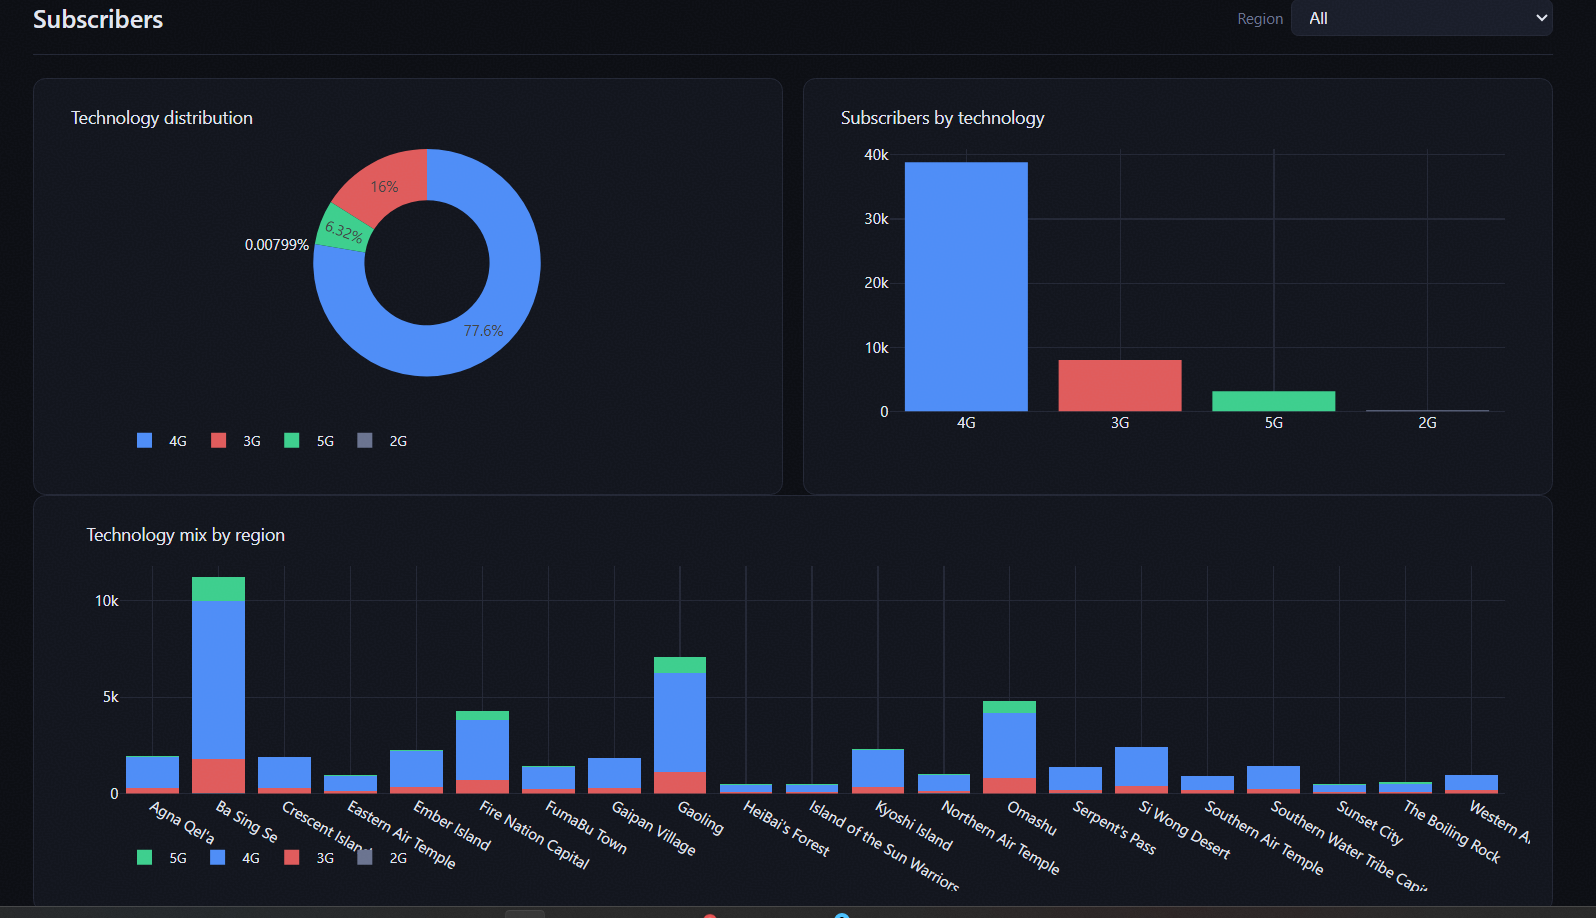
\includegraphics[width=0.85\textwidth]{figures/ch2-fictional-data.png}
\caption{Subscriber technology mix by region, from the live database. The region
names are fictional; the data behind them is internally consistent.}
\label{fig:ch2-fictional-data}
\end{figure}

\section{First Prototype: A Local Agent Loop}

With the databases in place, the next question was whether the actual
idea — ask a question in plain English, get a SQL-backed answer — could
work at all before worrying about making it fast or polished. The fastest
way to find out was to wire up a minimal agent loop against a model
running entirely locally, no cloud dependency, no API cost, nothing to
wait on.
\subsection{Getting a Loop Working}
The first version ran on Ollama~\cite{ollama} with a local qwen
model~\cite{qwen} — 7B, later bumped to 8B — driving a single-step
reasoning loop built around plain text tags rather than anything
structured: \ldots the model would read the question and respond with a \texttt{QUERY\_SC:} or \texttt{QUERY\_OP:}
tag followed by raw SQL, the loop would run that query against the
matching database, feed the result back, and repeat until the model
wrote a \texttt{CONCLUDE:} tag with its final answer. No tool-calling
API, no structured output — just a prompt format the model had to follow
by convention, parsed back out with regular expressions on this end.
For the first prototype we used a heavily customized Streamlit app
(Figure~\ref{fig:streamlit-prototype}) --- dark theme, custom fonts, a chat
panel next to a live snapshot area for charts. Streamlit handles layout and
reactivity on its own, so the time went into the agent loop rather than into
frontend code.

Simple and crude as it was, it did prove the core idea worked: the model could
turn a natural-language question into a query against the schema from
Section~\ref{sec:db-design}, chain a couple of query steps together when one
wasn't enough, and land on something coherent. That gave us a green light to
keep going down this path. The tag-based format itself stuck around much longer
than the local models did, and still shows up later in the report as the
fallback path once tool-calling was introduced.

But the very same screenshot also shows the limitations: the question asked for
a drilldown tree of technologies used against terminal capability, and the agent
answered with a dense block of raw counts --- while the ``Live Snapshot'' panel
next to it stayed completely empty. The reasoning loop could get the numbers
right, but numbers like these need to be visually accessible; a chart or a
drilldown tree would do a lot better. So that became another thing to fix.


\begin{figure}[H]
    \centering
    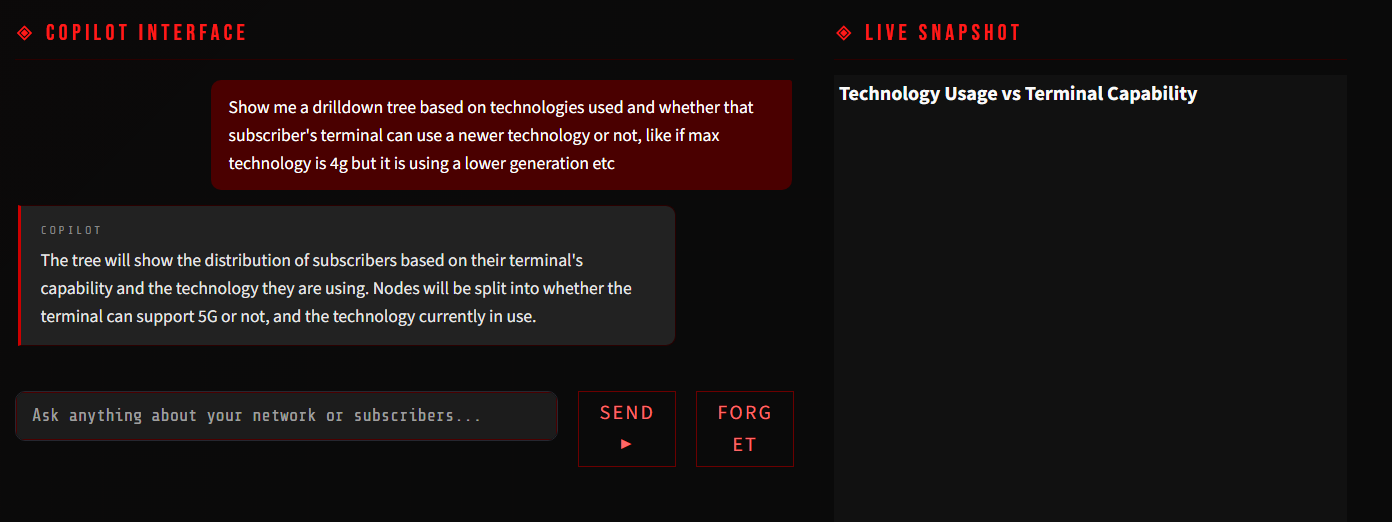
\includegraphics[width=0.9\textwidth]{figures/streamlit_prototype.png}
    \caption{The first Streamlit prototype: a drilldown-tree question answered
    with raw counts and no chart.}
    \label{fig:streamlit-prototype}
\end{figure}


\subsection{Hitting the Hardware Ceiling}

What that first loop did not prove was that local inference was viable to
actually use. It ran on an RTX 3050 with 4~GB of VRAM — enough to load a
7B–8B model, but not enough headroom to serve it at a usable latency once
the prompt included schema context and a few turns of conversation.

Every step of the loop meant another full model call, and with local inference
this slow, a question that should feel instant took far too long. The whole
point of the project was to ask a question and get a thorough answer, and
waiting minutes for one didn't make sense. The impasse was hardware, so we
started looking for alternatives.

\section{The Case for Cloud Inference}

One thing worked in favor of moving the reasoning off-device. Since the
environment was entirely synthetic from the start
(Section~\ref{sec:fictional-geography}), the usual objection to sending
data to a cloud-hosted model simply did not apply — there was no real
subscriber data to protect. That removed the main reason to keep
insisting on local inference, and made the switch a pragmatic step rather
than a fraught one.

Somewhere in the middle of babysitting local qwen3:8b through yet another
sluggish response — close to five minutes for a single prompt to come
back — the whole thing stopped feeling like an engineering trade-off and
started feeling like a bad idea. Both GPU and CPU were pinned the entire
time, since the model did not fit cleanly into 4~GB of VRAM and spilled
over onto the CPU, which raised a more immediate concern than ``is this
the right architecture'': at this rate, was this actually going to fry
the machine?

That is the point this got discussed with a colleague, who, on hearing
``five minutes per prompt,'' asked the obvious question: why not just use
something cloud-hosted instead?

Before that conversation, a local-but-not-quite-local option was briefly
on the table — spinning up a VM through Azure's student credit pack. However that idea
died quickly as the free-tier images do not come with a free GPU or VRAM attached, 
but maybe that was a blessing in disguise as eventually we came across a much more 
efficient solution.
My colleague then suggested using  AWS Bedrock~\cite{aws_bedrock}, which is Amazon's managed
access layer for foundation models. Getting access to \$100 of credit was actually pretty 
simple, I just needed a legitimate card entered, and from there, I got access to lots of 
models, which would normally require a lot of computational force, like qwen3 32B or 80B.
Answers were quick, more precise, and no hardware to worry about.


% =====================================================================
% SCREENSHOT NEEDED --- figures/ch3-bedrock-console.png
% Where: AWS Console -> Bedrock -> Model access (or the Bedrock
% playground/usage page).
% What to capture: the list of enabled foundation models (qwen3-32b /
% qwen3-next-80b-a3b should be visible as "Access granted"), ideally
% with the free usage credit balance visible somewhere on the page too.
% =====================================================================
\begin{figure}[htbp]
\centering
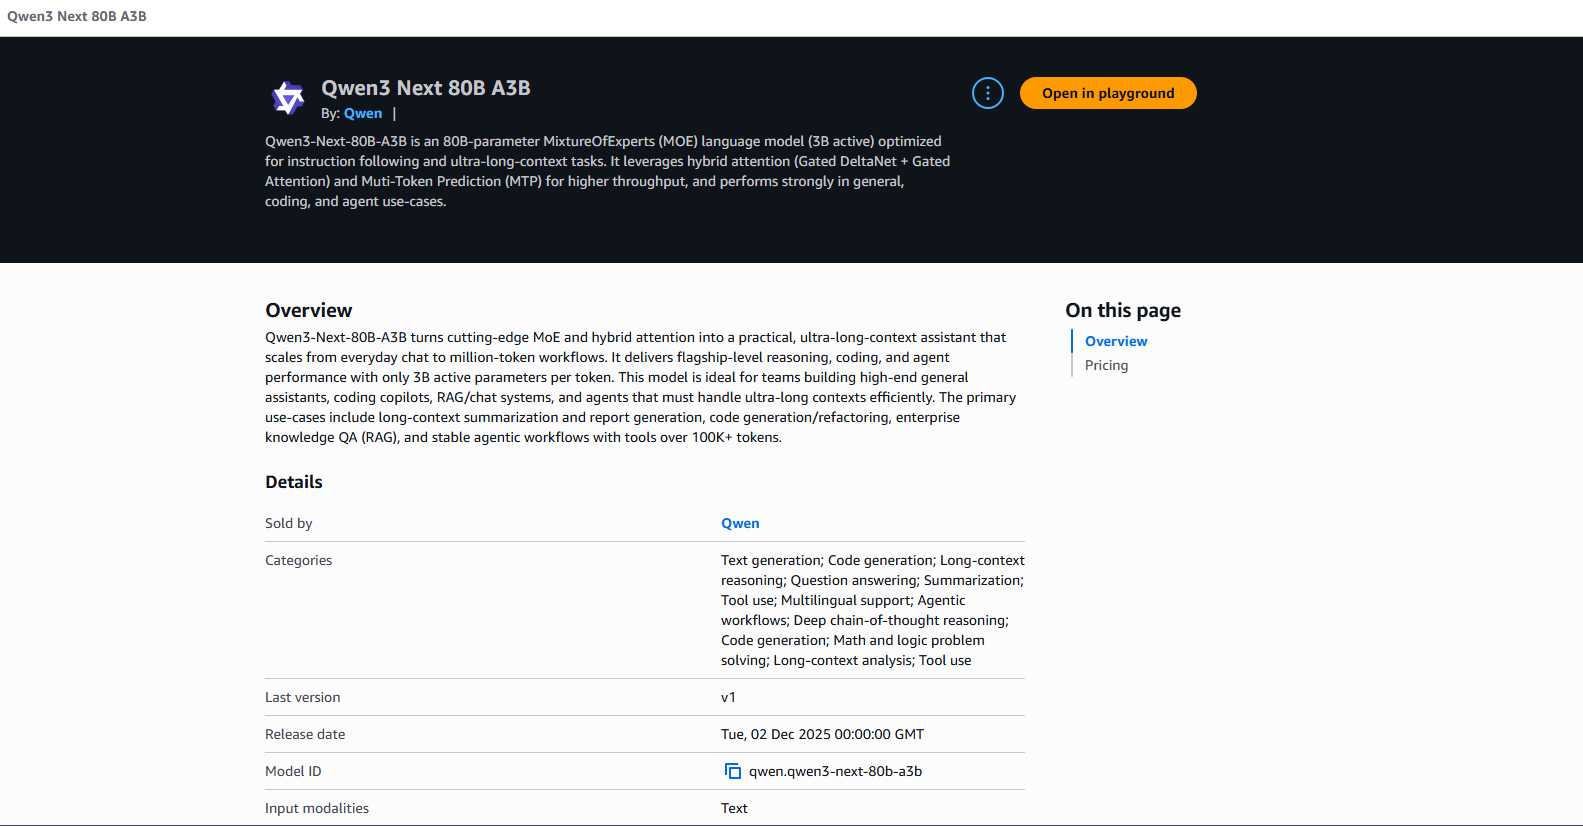
\includegraphics[width=0.85\textwidth]{figures/ch3-bedrock-console.png}
\caption{The AWS Bedrock console showing model access enabled for the
models used in this project.}
\label{fig:ch3-bedrock-console}
\end{figure}

\section{Cleaning Out the Local Stack}

Once cloud inference was clearly the model going forward, the local-model
code that had made up the entire agent up to this point turned into dead
weight rather than a fallback worth keeping around. After that, no more ollama startups, 
launching the server became faster and easier. The old code wasn't outright deleted but
rather archived for the record. 

\section{Making the Cloud Call Reliable}

A local model either answers or it crashes. A network call to a shared
API fails in a completely different way: throttling, timeouts, or the
odd server-side hiccup that has nothing to do with the question being
asked and everything to do with system load at that exact moment.
Treating every one of those as a hard failure would have made the agent
flaky in exactly the way switching to Bedrock was supposed to fix. So
the Bedrock call got wrapped in a retry layer instead: on a transient
error it backs off exponentially and tries again, up to four attempts,
and only retries when nothing had already streamed back so a partial
response never gets duplicated. Small piece of plumbing, but it is the
difference between the agent occasionally failing for no visible reason
and quietly recovering from the kind of hiccup any cloud API throws
from time to time.

% =====================================================================
% System architecture: processes, stores, and what talks to what.
% =====================================================================
\begin{figure}[H]
\centering
\definecolor{procblue}{HTML}{4A6FA5}
\definecolor{storebrown}{HTML}{B5793A}
\definecolor{extgreen}{HTML}{2E8B57}
\definecolor{busamber}{HTML}{C08A2E}
\resizebox{0.95\textwidth}{!}{%
\begin{tikzpicture}[
  proc/.style={rectangle, rounded corners=4pt, draw=procblue, very thick,
    fill=procblue!10, align=center, text width=3.4cm, inner sep=7pt,
    font=\bfseries\footnotesize},
  store/.style={cylinder, shape border rotate=90, aspect=0.22,
    draw=storebrown, very thick, fill=storebrown!12, align=center,
    text width=2.5cm, inner sep=5pt, font=\scriptsize},
  ext/.style={rectangle, rounded corners=4pt, draw=extgreen, very thick,
    fill=extgreen!10, align=center, text width=3.0cm, inner sep=7pt,
    font=\bfseries\footnotesize},
  bus/.style={rectangle, rounded corners=3pt, draw=busamber, very thick,
    fill=busamber!15, align=center, text width=4.0cm, inner sep=6pt,
    font=\scriptsize\ttfamily},
  user/.style={rectangle, rounded corners=3pt, draw=black!55, thick,
    fill=black!5, align=center, text width=2.9cm, inner sep=6pt,
    font=\footnotesize},
  lbl/.style={font=\scriptsize\itshape, align=center, inner sep=2pt},
  flow/.style={-{Latex[length=2.4mm]}, thick},
  biflow/.style={{Latex[length=2.4mm]}-{Latex[length=2.4mm]}, thick},
]

% ---- nodes, placed on explicit coordinates ----
\node[user]  (browser) at ( 0,   0)    {Operator\\[1pt]\normalfont\scriptsize web browser};
\node[proc]  (chat)    at ( 0,  -2.0)  {Chat Server\\[2pt]\normalfont\scriptsize server.py : 8000};
\node[ext]   (bedrock) at ( 6.4,-2.0)  {AWS Bedrock\\[2pt]\normalfont\scriptsize qwen3-32b / 80b-a3b};
\node[proc]  (agent)   at ( 0,  -4.2)  {Reasoning Agent\\[2pt]\normalfont\scriptsize tool loop, grounding,\\verification};

\node[proc]  (sim)     at (-6.9,-7.0)  {Simulator\\[2pt]\normalfont\scriptsize db\_simulator.py\\one tick / 30 s};
\node[store] (scdb)    at (-2.9,-7.0)  {NetworkAnalyzer\\\_new.db\\[2pt]\itshape network};
\node[store] (opdb)    at ( 2.9,-7.0)  {operator\\\_new.db\\[2pt]\itshape commercial};
\node[proc]  (dash)    at ( 6.9,-7.0)  {Dashboard\\[2pt]\normalfont\scriptsize dashboard\_server.py\\: 8002};

\node[bus]   (mqtt)    at ( 0,  -9.8)  {MQTT broker : 1883\\[1pt]\rmfamily networkanalyzer/actions/\#};
\node[proc]  (ops)     at ( 0, -11.6)  {Ops Portal\\[2pt]\normalfont\scriptsize ops\_server.py : 8001};
\node[user]  (human)   at ( 0, -13.4)  {Human reviewer\\[1pt]\normalfont\scriptsize approve / edit / reject};

% ---- edges ----
\draw[biflow] (browser) -- node[lbl,right]{question / answer} (chat);
\draw[biflow] (chat) -- node[lbl,above]{tool calls} (bedrock);
\draw[flow]   (chat) -- (agent);

\draw[biflow] (agent.south) -- ++(0,-0.6) -| (scdb.north);
\draw[biflow] (agent.south) -- ++(0,-0.6) -| (opdb.north);

\draw[flow] (sim.east) -- node[lbl,above]{writes} (scdb.west);
\draw[flow] (sim.south) -- ++(0,-1.1) -| (opdb.south);

\draw[flow] (scdb.east) -- ++(0.5,0) |- (dash.west);
\draw[flow] (opdb.east) -- node[lbl,above]{reads} (dash.west);
\draw[flow] (dash.north) |- ++(0,1.4) -| node[lbl,above right]{charts} (browser.east);

\draw[flow] (agent.south) -- ++(0,-0.6) -- (0,-9.0) -- node[lbl,right]{propose\_action} (mqtt.north);
\draw[flow] (mqtt) -- node[lbl,right]{subscribe} (ops);
\draw[biflow] (ops) -- node[lbl,right]{review queue} (human);
\draw[flow] (ops.east) -- ++(1.6,0) |- node[lbl,below right, text width=2.6cm]{written only after approval} (opdb.south east);

\end{tikzpicture}%
}
\caption[End-to-end system architecture]{End-to-end system architecture: five
processes sharing two SQLite files, with every outward-facing action routed
through the message bus and a human reviewer.}
\label{fig:architecture}
\end{figure}

\section*{Conclusion}

This chapter laid the foundation everything else in this report builds on:
two SQLite databases, joined on \texttt{msisdn}, split along the same
network/commercial line real operators use, populated with
\textasciitilde50{,}000 synthetic but internally consistent subscribers
across a fictional geography. On top of that data, a first agent loop
proved the core idea could work — but running it on a local 7B–8B model
made clear that hardware was going to be the limiting factor, not the
idea itself.

That's what prompted the move off local inference entirely. An 8B model could
get the numbers right, but five minutes per question while pinning both GPU and
CPU was never going to work. We tested Bedrock first at 32B, then settled on the
80B model, keeping 32B around for when speed mattered more. From there the old
local-model code was cleaned out rather than kept as a fallback, and the API
call itself was hardened against the transient failures any cloud service
produces.

Before getting into what the agent built on top of this call can actually do,
the next chapter covers what it works against --- a database that never sits
still.

\addcontentsline{toc}{section}{Conclusion}



\chapter{A Living Database}\label{ch:livingdb}

\section*{Introduction}
\addcontentsline{toc}{section}{Introduction}

Every chapter so far has treated the database as a fixed thing sitting
underneath the agent: a schema to design, a set of tables to query. It
never actually is one. From the first tick after the server starts, a
separate process is quietly rewriting both databases underneath
whatever the agent is doing --- shifting KPIs, opening and healing
service incidents, accumulating usage, recomputing churn scores,
occasionally creating a brand-new subscriber out of nowhere. The agent
in the next chapter is built entirely around the assumption that this
is true: that the world it is answering questions about is not sitting
still, and that nothing it has already said can be trusted to still be
correct a few minutes later. Before getting into what the agent can do
with that world, this chapter covers what the world itself actually
does on its own.

\section{Why a Static Database Was Never Going to Be Enough}
The database created from Chapter 
The synthetic databases from Chapter~\ref{ch:database} gave the project
something to query, but a database that only changes when someone re-runs a
generation script is just a snapshot. Real networks don't sit still, so ours
shouldn't either. There's a less obvious reason too: if the numbers never move,
an agent that quietly memorized its first answer looks exactly as correct as one
that queries the database honestly every time. A moving target is the only way
to tell those two apart --- which is what \texttt{db\_simulator.py} is for.

\section{The Tick Loop}

\texttt{db\_simulator.py} runs as its own long-lived process, entirely
separate from the chat server, and advances the environment forward on
a fixed schedule --- one \emph{tick} every few minutes. Each tick walks
through a set of update functions, and each one touches a different
slice of the two databases:

\begin{itemize}
    \item \textbf{KPIs and alarms} --- network performance metrics
    (throughput, latency, drop rate) get nudged, faults get raised on
    cells, and the two are wired to each other in both directions
    (Figure~\ref{fig:ch4-alarms}).
    \item \textbf{Usage} --- this updates montly data and voice usage for a rotating
    number of subscribers, relatively like real usage would build up gradually over
    the course of a month, rather than getting an impulse.
    \item \textbf{Churn rescoring} --- every affected subscriber's
    churn risk gets calculated again, based on their latest activities, and 
    how network KPIs affect thenm, not left stale from whenever it was last 
    calculated.
    \item \textbf{New subscribers} --- occasionally, the database may get or lose 
    a new subscriber, it gets created from scratch and added to both databases at once, so the 
    50{,}000 isn't a fixed number either.
    \item \textbf{The calendar} --- the simulator keeps its own notion
    of ``today,'' and that notion advances tick by tick independently
    of the real-world date. A month can complete and roll over inside
    the simulation without the actual calendar moving at all.
\end{itemize}

% =====================================================================
% SCREENSHOT NEEDED --- figures/ch4-alarms.png
% Where: analytics dashboard (localhost:8002), Network section.
% What to capture: the KPI trend chart together with the active alarms
% list/table, showing both a chart (built from kpis_daily) and a set of
% currently-raised alarms in the same view.
% =====================================================================
\begin{figure}[H]
\centering
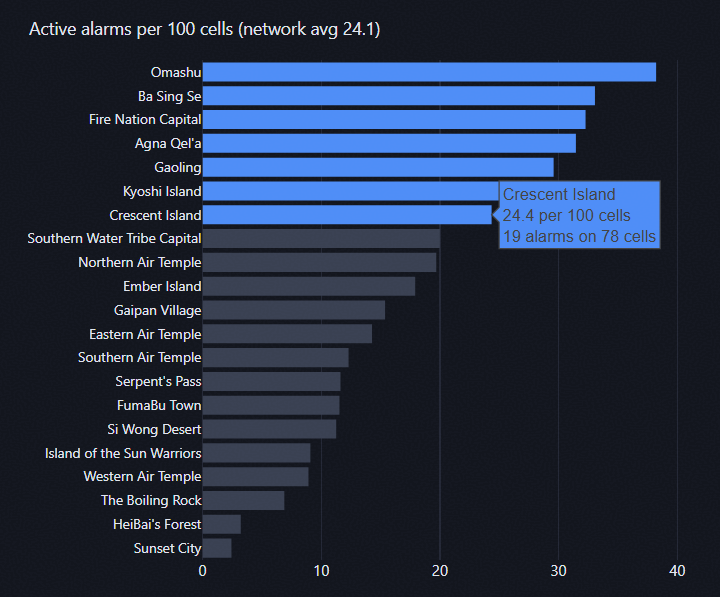
\includegraphics[width=0.85\textwidth]{figures/ch4-alarms.png}
\caption{Active alarms per 100 cells by region, from live simulator data.
Omashu leads once normalized.}

\label{fig:ch4-alarms}
\end{figure}

These updates aren't dramatic on their own, but with enough time, it accumulates a more 
interesting result, asking the agent the same question a minute apart won't change much,
but an hour, it'll show significant change, something a static database could never offer.


% =====================================================================
% SCREENSHOT NEEDED --- figures/ch4-simulator-tick.png
% Where: terminal running db_simulator.py directly (python db_simulator.py).
% What to capture: a few consecutive tick log lines showing the kind of
% updates it applies each cycle (KPI updates, alarms, churn rescoring,
% new-incident lines, etc.) --- enough to show it is a continuously
% running process ticking forward, not a one-shot script.
% =====================================================================
\begin{figure}[H]
\centering
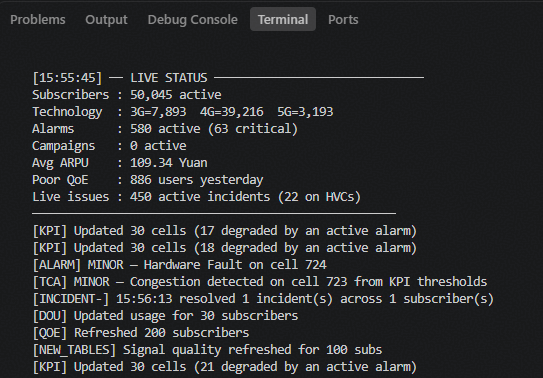
\includegraphics[width=0.85\textwidth]{figures/ch4-simulator-tick.png}
\caption{\texttt{db\_simulator.py} running its tick loop, continuously updating
both databases while the agent stays live.}
\label{fig:ch4-simulator}
\end{figure}

\section{Live Service Incidents: Open, Spread, Heal}

The most involved piece of the simulator is not a background metric
drifting slightly --- it is a full incident lifecycle, built so the
agent can be asked something like ``do we have any high-value
customers having streaming issues right now'' and get a real, current,
truthful answer.
Every incident lives in an \texttt{experience\_incidents} table, it has a root 
cause, an affected service, a severity and a full timestamp trail. But one incident
can't really be a lone flag on a row: opening one also lays down a run of poor 
QoE scores for that service, a matching service-interruption, and, if it's serious enough,
a customer complaint is also filed. 
. Asking the agent to explain \emph{why} a
customer's experience looks bad is meant to hold together as a story,
not just a single suspicious number.

\subsection{Blast Radius: Not Every Fault Hits One Customer}

An early version of this feature made every incident purely
per-customer, and it produced a result that did not survive a second
look: a ``critical power failure at a site'' that supposedly affected
exactly one subscriber, when that site was actually serving over fifty
people. The fault itself was real and correctly reported by the agent
--- the problem was in the data, not the reasoning built on top of it,
which is precisely why it is worth naming here rather than in the next
chapter: it was a modeling gap in the simulator, not a mistake by the
agent.

The fix was to give every incident a defined \emph{scope}, matching how
that class of fault actually behaves in a real network:

\begin{table}[H]
\centering
\small
\begin{tabular}{@{}p{3.1cm}p{4.9cm}p{5.4cm}@{}}
\toprule
\textbf{Scope} & \textbf{Who it affects} & \textbf{How the simulator picks it} \\
\midrule
\textbf{Site}\newline{\footnotesize power failure, site outage}
& Every active subscriber on every cell at that site
& \(\sim\)2\% of new incidents --- an outage that big is rare \\
\addlinespace
\textbf{Cell}\newline{\footnotesize congestion, backhaul degradation, interference}
& Every active subscriber on that cell
& Weighted toward busier cells, where congestion actually happens \\
\addlinespace
\textbf{Subscriber}\newline{\footnotesize throttling, DNS or CDN hiccup, dropped VoLTE bearer}
& One customer
& Biased toward high-value subscribers \\
\bottomrule
\end{tabular}
\caption{Incident scopes and how the simulator selects them.}
\label{tab:incident-scopes}
\end{table}

``High-value'' here is not a fixed ARPU threshold but the top decile of the live
distribution, re-tested as revenue moves --- so the label keeps meaning
something even as ARPU drifts

Once a site- or cell-scoped incident fires, every subscriber caught in
its blast radius gets a consistent snapshot of the incident attached to
their record --- so a question filtered to high-value customers only
returns the high-value customers genuinely inside that radius, not
everyone the fault happened to touch. A power failure at a site serving
mostly bronze-tier subscribers in a poorer part of the fictional map
and one serving mostly platinum subscribers in a wealthier one are the
same fault with completely different commercial urgency, which is
exactly the distinction a purely per-customer model could never have
produced.

\subsection{Self-Healing}

An incident does not sit open forever. Every tick, a separate resolution
pass checks every active incident against the \texttt{expected\_}
\texttt{resolution\_at} timestamp it was given at open, and closes
anything past due: status flips to resolved, \texttt{resolved\_at} gets
stamped, and any linked complaint gets marked resolved too. The row
itself is never deleted, so a question like ``what happened to this
customer at 14:32 today'' still has a real answer to give hours or days
later --- the incident heals, but the history of it having happened
does not disappear with it.

\section{Alarms That Actually Mean Something}

The blast-radius problem had a sibling that hid for much longer. Alarms
and KPIs both looked fine on their own --- the alarms table filled up,
the KPI numbers moved --- so neither invited a second look. But the issue is 
that they never linked/synced with each other, this means that each tick raised
an alarm on a cell picked randomly, wrote the row, and stopped there, while 
the KPI generator rolled its own seperate dice and never read the alarms this table.
The giveaway was clear in the data though: cells carrying an active \emph{critical}
alarm measured a slightly \emph{lower} drop rate than cells with no alarm at all.
This of course made no sense and had to be fixed. And since cells were picked from the whole network rather than
the parts of it serving people, 62\% of alarms sat on cells with zero
subscribers on them.


Fixing it meant wiring the two together in both directions, because
real faults work both ways. Equipment faults --- a power failure, a
hardware fault, a backhaul link going down --- announce themselves, and
the degraded counters follow as a consequence. Performance faults are
the reverse: congestion, interference and coverage holes have no box to
raise a flag, and the only way anyone finds out is by watching the
counters cross a threshold, which is what a real network management
system calls a threshold-crossing alert. So a raised fault now degrades
the cell it sits on --- each fault type hitting the metric it would
actually hit, scaled by severity --- and opens real incidents for the
customers on that cell if it is serious enough, feeding the same
evidence trail and churn coupling described above. Running the other
way, a detector reads each cell-day and raises the alarm those numbers
deserve.

One detail there is worth keeping, because the obvious approach fails
quietly. Thresholds need to relative to the technology and not absolute: a 
1.9\% drop rate is a broken 5G cell and a completely ordinary 2G one. A flat ``
drop rate above 2\%'' rule currently flags 188 2G cells, 45 for 3G and 50 for 
4G, and not one of those 2G is under an alarm, while the 4G ones, all of them are 
under an alarm. So the rule works and does find real faults, and then buries them
under nearly four times as many cells whose only crime is being 2G.
Every threshold is therefore expressed against that technology's own
healthy baseline.

One bug is worth admitting: the KPI update function had never written a single
row. Its upsert depended on a uniqueness constraint the table didn't have, the
database helper swallowed the error, and the function went on reporting success
every tick. The helpers now print real errors instead of retrying past them.
With that fixed, cells under an active alarm run 1.4 to 2.1 times the drop rate
of clean cells, and 1{,}089 of 1{,}099 active alarms sit on a cell that actually
serves somebody.


\section{Churn Tracks the Live World, Not Just Usage}

Churn risk here is the sum of two parts, computed separately on purpose. The
first is a baseline from a subscriber's own commercial behaviour --- spend
falling against their own history, bills going unpaid, usage tailing off, a short
tenure. The second is a penalty from what is happening to them on the network
right now. Chapter~\ref{ch:eval} covers how that baseline is computed and why it
ended up as an explainable scorecard rather than the machine-learning model
originally trained for it.

The reason for splitting them is that a baseline built from monthly commercial
history has no way of reacting to something happening to a customer
\emph{today}. The live incident log closes that gap: every affected subscriber
is rescored the moment an incident opens against them, with a penalty added on
top of the baseline, driven by how many active incidents and unresolved
complaints they currently have. Once the incident heals, the next rescoring pass
lets that penalty relax back down.

So a platinum subscriber sitting on a comfortable, low-risk baseline can be
pushed into a genuinely elevated risk band for as long as their streaming
service is actually degraded, and settle back down once it recovers --- churn
risk that tracks the live state of the world, rather than a number computed once
and left to go stale. The two halves are kept strictly separate: the baseline
never reads incidents, and the penalty never reads commercial history, so
neither signal is counted twice.

\section{Seeing It on the Map}
The coverage map associated to the work is not just a static look, it
represents multiple things: the cell site locations, showing density in 
certain cities, as well as current alarms, clicking on a ring will immediately
prompt the agent to investigate the said alarm, searching up root cause as well as suggesting solutions.


% =====================================================================
% SCREENSHOT NEEDED --- figures/ch4-map-flash.png
% Where: chat UI (localhost:8000), Coverage tab in the snapshot panel.
% What to capture: the map with at least one pulsing incident ring
% visible, ideally with the hover tooltip open showing the site/service/
% severity details. If you can catch the "Issues only" toggle active
% too, even better --- otherwise a normal view with rings is enough.
% =====================================================================
\begin{figure}[H]
\centering
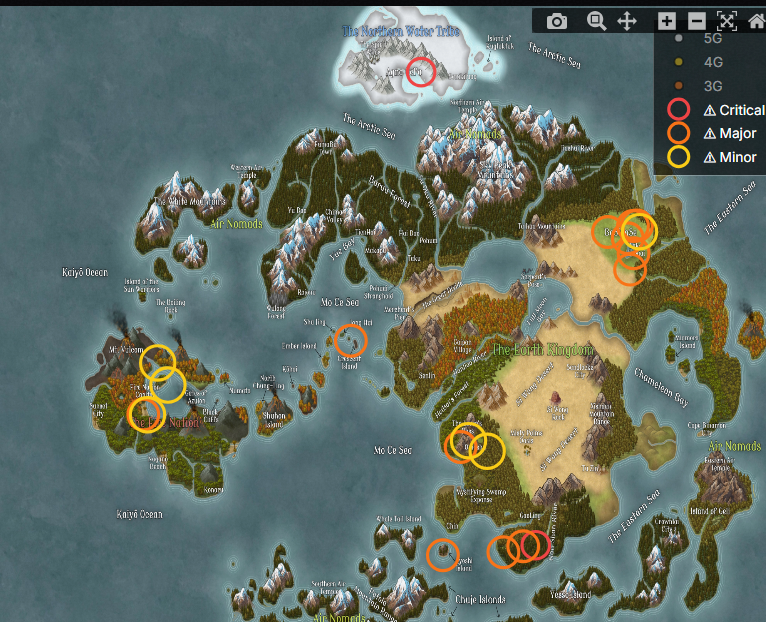
\includegraphics[width=0.85\textwidth]{figures/ch4-map-flash.png}
\caption{The coverage map flashing a live incident, colored and pulsing
by severity, driven directly by the active rows in
\texttt{experience\_incidents}.}
\label{fig:ch4-map-flash}
\end{figure}

\section{The Partial-Month Gotcha}

Because monthly usage figures accumulate tick by tick over the course
of a simulated month rather than existing fully formed from day one,
there is a real and slightly counterintuitive consequence worth naming
directly: a question asked on the second day of a new simulated month
legitimately returns a much smaller number than the exact same question
asked on the last day of the previous one. When read in isolation, a ``
top data user this month'' answer of a few gigabytes early in a cycle 
can look like the agent got it wrong, when in reality, it was the correct 
answer, just not logically. This came up directly while testing: an 
answer citing a small usage figure for a specific subscriber 
looked like the number was hallucinated at first glance, but checking the 
database it was correct, as the month had just begun.  Knowing the data is
genuinely live --- not stale, not wrong, just incomplete for the
current period --- is what keeps a correct answer from being misread
as a bug.

\section*{Conclusion}
\addcontentsline{toc}{section}{Conclusion}

This chapter covered the piece of the project that everything else
quietly depends on: a database that never actually holds still.
\texttt{db\_simulator.py} advances KPIs, usage, and the subscriber base
tick by tick, but the real weight of the chapter is the incident
lifecycle built on top of it --- faults that open with a real cause, a
proportionate blast radius instead of a flat per-customer model, and a
resolution path that lets them heal on their own, all of it feeding
directly into churn scoring and the live coverage map. None of this
exists for its own sake. It exists so that the agent, covered in the
next chapter, cannot get away with memorizing an answer and repeating
it --- every claim it makes has to survive being checked against
whatever the database currently says, because the database it is
reading from is not the same one it was reading from five minutes ago.

\chapter{How the Agent Works}\label{ch:agent}

\section*{Introduction}
\addcontentsline{toc}{section}{Introduction}

A capable model on its own does not solve the actual problem. Handed a
question like ``which regions have upsell opportunity for 5G,'' qwen3
cannot just answer. It does not know the schema, it cannot see the
database, and even if it could write one correct query, plenty of real
questions need more than one query chained together before there is
enough to answer from. So what actually turns a single model call into
something that can do that? The loop wrapped around it: read the
question, decide on an action, observe what came back, and either take
another action or conclude. And that loop is not new to this chapter ---
it is the exact same idea the first local prototype in Chapter~\ref{chapter:BF-DFP} was
already built around. What changed between then and now is not the
architecture, it is how reliably the model's chosen action gets
communicated back to the code running it. There is also a difference in
what the loop is running against: the previous chapter established that
the database underneath it never sits still, so everything the agent
does here --- every query, every chart, every exported row --- is read
against a target that is actively moving, not a fixed snapshot. This
chapter covers how that loop actually works today, how it grounds
itself in the real schema instead of guessing, how it catches its own
mistakes before they reach the user, and everything it can do beyond
just answering in text. And it is worth flagging what to watch for while reading
it. Chapter~\ref{ch:context}, Section~\ref{sec:challenges}, laid out three gaps
that started this whole project off: raw data that never quite becomes actionable
insight, churn scores that live somewhere the people who need them do not look,
and a wait between asking a business question and getting an answer backed by
real data. Everything from here on is those three being handled one at a time, so
it is worth keeping them in mind as each piece goes past.

\section{The Loop: One Consistent Idea, Two Implementations}

Strip away everything specific to Bedrock or tool-calling, and the
agent's architecture is the same simple cycle it has been since
Chapter~\ref{chapter:BF-DFP}: \emph{perceive, decide, act, observe, repeat} --- read the
question and whatever has been learned so far, decide on exactly one
action, take it, look at what came back, and either take another action
or conclude with a final answer. This is the same reason-act-observe
pattern behind the ReAct approach to language-model agents~\cite{react}:
interleaving reasoning steps with concrete actions against the outside
world, rather than asking the model to reason its way to an answer in
one shot. Figure~\ref{fig:agent-loop} shows this cycle as it runs today.

What actually changed between the local Ollama prototype and the
current agent is not this cycle, but how an ``action'' gets expressed
and recognized. In Chapter~\ref{chapter:BF-DFP}, the model wrote a plain-text tag ---
\texttt{QUERY\_SC:}, \texttt{QUERY\_OP:}, or \texttt{CONCLUDE:} ---
followed by whatever it wanted to run or say, and the code on this end
parsed it back out with regular expressions. It worked, however nothing 
forced the model to follow that format specifically, as it drifts slightly to 
the step failed, without any clean way for the loop to recover.

To solve that issue, Bedrock's tool calling replaced the convention with a schema: a
fixed set of tools, each having an input shape, validated by the API before the loop sees anything:

\begin{itemize}
    \item \texttt{run\_sql(database, query)} --- execute a SQL query
    against the network or commercial database and return the rows.
    \item \texttt{inspect\_schema(table)} --- look up the real columns
    of a table before writing a query against it, rather than guessing.
    \item \texttt{conclude(text, recommendations, chart, ...)} --- end
    the loop with a final answer, optionally attaching a chart,
    recommendations, or a visualization spec.
    \item \texttt{propose\_action(description)} --- instead of
    answering, propose an operational action (a campaign, an SMS, a
    network flag) for a human to review, rather than taking it directly.
\end{itemize}

The loop itself did not need to change to adopt this --- it still asks
``what is the next action,'' takes it, and observes the result. What
changed is that ``the next action'' is now a structured tool call
instead of a string that has to be hoped for and parsed, which is what
makes the whole system meaningfully more reliable than the Chapter~\ref{chapter:BF-DFP}
version, not a difference in the underlying idea.

\begin{figure}[H]
\centering
\definecolor{agentblue}{HTML}{4A6FA5}
\definecolor{toolgray}{HTML}{6B7280}
\definecolor{concgreen}{HTML}{2E8B57}
\definecolor{actamber}{HTML}{B5793A}
\resizebox{\textwidth}{!}{%
\begin{tikzpicture}[
  qbox/.style={rectangle, rounded corners=3pt, draw=black!60, thick,
    fill=black!4, align=center, text width=4.4cm, inner sep=8pt, font=\footnotesize},
  agentbox/.style={rectangle, rounded corners=4pt, draw=agentblue, very thick,
    fill=agentblue!10, align=center, text width=5.6cm, inner sep=10pt, font=\bfseries\footnotesize},
  toolbox/.style={rectangle, rounded corners=3pt, draw=toolgray, thick,
    fill=toolgray!8, align=center, text width=4.6cm, inner sep=7pt, font=\footnotesize\ttfamily},
  obsbox/.style={rectangle, rounded corners=3pt, draw=toolgray, thick,
    fill=toolgray!15, align=center, text width=6.2cm, inner sep=7pt, font=\footnotesize},
  concbox/.style={rectangle, rounded corners=3pt, draw=concgreen, thick,
    fill=concgreen!10, align=center, text width=4.6cm, inner sep=7pt, font=\footnotesize\ttfamily},
  ansbox/.style={rectangle, rounded corners=3pt, draw=concgreen, very thick,
    fill=concgreen!18, align=center, text width=4.6cm, inner sep=8pt, font=\bfseries\footnotesize},
  actbox/.style={rectangle, rounded corners=3pt, draw=actamber, thick,
    fill=actamber!12, align=center, text width=4.6cm, inner sep=7pt, font=\footnotesize\ttfamily},
  humbox/.style={rectangle, rounded corners=3pt, draw=actamber, very thick,
    fill=actamber!20, align=center, text width=4.6cm, inner sep=8pt, font=\bfseries\footnotesize},
  lbl/.style={font=\scriptsize\itshape, align=center},
]

\node[qbox] (q) {User Question\\[2pt]\normalfont\scriptsize (plus anything already learned this turn)};
\node[agentbox, below=9mm of q] (agent) {Agent\\[2pt]\normalfont\footnotesize reasons over the question and decides exactly one next action};

\node[toolbox, below=16mm of agent, xshift=-6.2cm] (runsql) {run\_sql(\allowbreak database,\allowbreak query)};
\node[toolbox, right=8mm of runsql] (inspect) {inspect\_schema(\allowbreak table)};
\node[obsbox, below=8mm of $(runsql.south)!0.5!(inspect.south)$] (observe) {Observe: query results, or the real columns of a table};

\node[concbox, below=16mm of agent, xshift=6.2cm] (conclude) {conclude(\allowbreak text,\allowbreak chart,\allowbreak ...)};
\node[actbox, right=8mm of conclude] (propose) {propose\_action(\allowbreak description)};
\node[ansbox, below=8mm of conclude] (answer) {Final Answer\\[2pt]\normalfont\footnotesize shown to the user};
\node[humbox, below=8mm of propose] (human) {Human Review\\[2pt]\normalfont\footnotesize (Ops Portal)};

% forward flow
\draw[-{Latex[length=2.5mm]}, thick] (q) -- (agent);
\draw[-{Latex[length=2.5mm]}, thick] (agent.south) -- ++(0,-4mm) -| (runsql.north);
\draw[-{Latex[length=2.5mm]}, thick] (agent.south) -- ++(0,-4mm) -| (inspect.north);
\draw[-{Latex[length=2.5mm]}, thick] (runsql.south) -- (observe.north -| runsql.south);
\draw[-{Latex[length=2.5mm]}, thick] (inspect.south) -- (observe.north -| inspect.south);
\draw[-{Latex[length=2.5mm]}, thick] (agent.south) -- ++(0,-4mm) -| (conclude.north);
\draw[-{Latex[length=2.5mm]}, thick] (agent.south) -- ++(0,-4mm) -| (propose.north);
\draw[-{Latex[length=2.5mm]}, thick] (conclude) -- (answer);
\draw[-{Latex[length=2.5mm]}, thick] (propose) -- (human);

% the loop-back — this is the actual cycle
\draw[-{Latex[length=2.5mm]}, thick, agentblue]
  (observe.west) to[out=180, in=270] node[lbl, agentblue, xshift=-2mm] {repeat until\\ready to conclude}
  ++(-2.6cm, 1.8cm) |- (agent.west);

\end{tikzpicture}%
}
\caption{The agent's reasoning loop. \texttt{run\_sql} and
\texttt{inspect\_schema} feed back into another round of reasoning;
\texttt{conclude} and \texttt{propose\_action} end it.}
\label{fig:agent-loop}
\end{figure}


\begin{figure}[H]
\centering
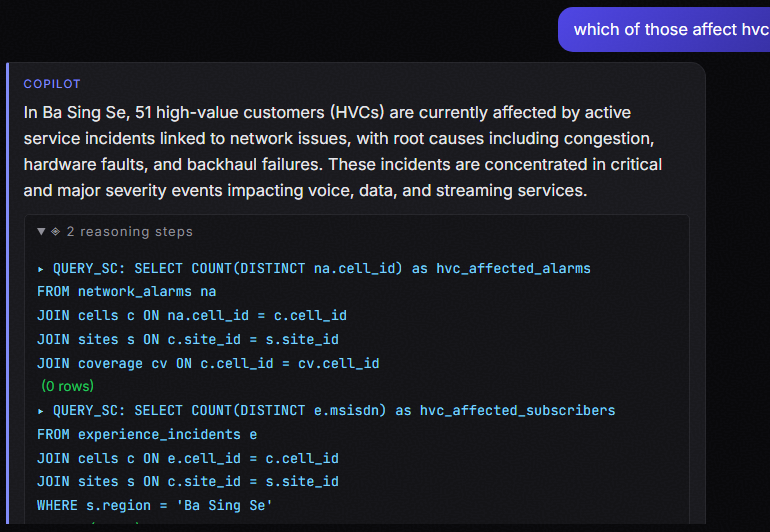
\includegraphics[width=0.8\textwidth]{figures/ch5-steps-panel-b.png}
\caption{The steps panel under a finished answer. The first \texttt{run\_sql}
returned no rows and is left visible rather than hidden.}
\label{fig:ch5-steps-panel}
\end{figure}

Figure~\ref{fig:agent-loop} is the theory. Figure~\ref{fig:ch5-steps-panel}
is what it actually looks like when the loop runs against a real
question --- every \texttt{run\_sql} step gets logged and shown to the
user, so the loop is not a black box even though the reasoning behind
each step is not shown in full.
\section{Knowing When Not to Answer Yet}

The first decision the loop makes is not which query to run. It is whether
the question can be answered honestly as asked.

Take a question the dashboard gets constantly: ``5G upsell opportunities
by region.'' That sounds specific enough. It is not. Does it mean every
subscriber holding a 5G-capable handset who is still on a 4G plan? Only
the high-value ones, because a campaign budget is finite? Only the ones
who are also showing churn risk, because those are the ones worth
spending a retention offer on? Those are three different lists, three
different campaigns, and three different costs. An agent that quietly
picks one and answers looks confident and is probably answering a
question nobody asked --- and, worse, the answer gives no clue which
reading it used.

So before running anything, the agent checks whether it should ask first.
Three gates, cheapest first, and most questions pass straight through all
three without paying for any of them:

\begin{table}[H]
\centering
\small
\begin{tabular}{@{}p{2.9cm}p{4.5cm}p{5.0cm}@{}}
\toprule
\textbf{Trigger} & \textbf{Looks like} & \textbf{What the agent does} \\
\midrule
Threshold only a human can set
& ``high ARPU'', ``heavy data users'', ``above average''
& Asks for a number, with a ``pick a sensible one for me'' fallback \\
\addlinespace
Breakdown with no dimension
& ``show me a drilldown of subscribers''
& Offers the real drill paths --- region, technology, value segment \\
\addlinespace
Genuine vagueness
& ``what should we focus on'', ``biggest problems''
& Asks the model what is actually being requested \\
\bottomrule
\end{tabular}
\caption{The three cases where the agent asks before it queries.}
\label{tab:clarify-gates}
\end{table}


% =====================================================================
% SCREENSHOT NEEDED --- figures/ch5-clarify.png
% Where: chat UI (localhost:8000), Copilot tab.
% What to capture: ask "5G upsell opportunities by region" and capture the
% clarify card BEFORE clicking an option --- the question the agent asks
% plus the list of option buttons, ideally with the answer that follows
% after picking one visible underneath.
% =====================================================================
\begin{figure}[H]
\centering
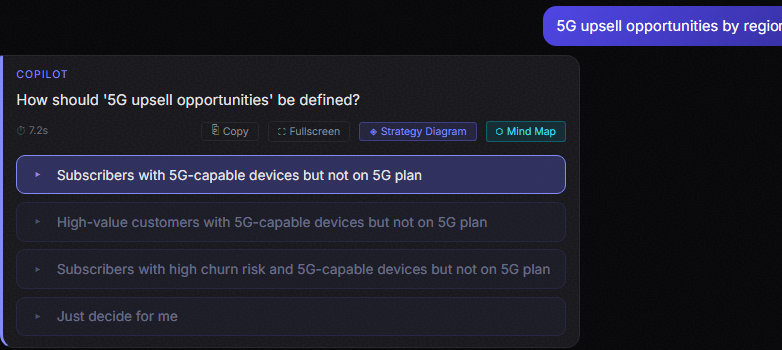
\includegraphics[width=0.85\textwidth]{figures/ch5-clarify1.png}
\caption{The agent declining to guess: three readings offered for ``5G upsell
opportunities by region'' before any query runs.}
\label{fig:ch5-clarify-ask}
\end{figure}

\begin{figure}[H]
\centering
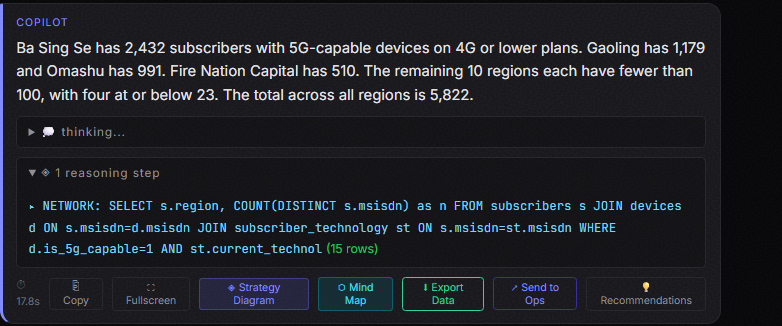
\includegraphics[width=0.85\textwidth]{figures/ch5-clarify2.png}
\caption{The answer, once a reading is chosen.}
\label{fig:ch5-clarify-answer}
\end{figure}


There are two details that make it behave like a tool/agent rather than 
a chatbot answering simple questions.


The options are \emph{complete standalone questions}, not dialogue turns.
Clicking ``High-value customers with 5G-capable devices but not on 5G
plan'' runs exactly that, as though it had been typed. There is no
half-remembered state waiting to be resumed, and nothing to go stale if
the user wanders off and asks something else instead. It also removes an
obvious way to build an infinite loop: the agent remembers which options
it just offered, so a clicked option runs directly instead of tripping
the same gate again and being asked to clarify its own clarification.

And the agent never asks the user to define a term the data already
defines. ``High-value customer'' is not a matter of opinion here --- it
is a column. Neither is ``having an issue right now,'' which is a row in
the live incident log with a timestamp on it. Questions like ``do we have
any HVCs with streaming issues right now'' therefore skip the whole gate
and run immediately, because every term in them is already pinned down by
the schema. Asking about those would not be careful, it would be
annoying.

The pattern here is the same one that runs through the rest of this
chapter. An agent that guesses and sounds certain is worse than one that
admits the question has more than one reading, in exactly the way an
answer built on numbers it never queried is worse than one that says it
does not know.

\section{Grounding the Agent in Domain Knowledge}

Knowing the four tools is one thing. Knowing which columns actually
exist in a twenty-plus table schema, or which of the two databases a
given question even belongs to, is another. So where does that
knowledge come from, if not from the model just knowing it?

Two different mechanisms, doing two different jobs, kept deliberately
separate. The first is a set of fixed behavioral rules baked directly
into the system prompt --- for example, a ranking principle that tells
the agent to compute every metric in one grouped query and never rank
by one number while quoting another. These are general, apply to every
question, and exist to fix \emph{reasoning} mistakes.

The second is retrieval: the same retrieval-augmented generation idea
behind giving a language model access to an external knowledge source
instead of relying purely on what it already knows~\cite{rag}, applied
here to schema and SQL knowledge rather than open-domain text. A schema
knowledge graph only injects the subgraph of tables and join paths
relevant to the current question, an intent classifier routes a
question toward the network side, the commercial side, or both, and a
hybrid search index --- BM25~\cite{bm25} keyword matching and FAISS-based
vector search~\cite{faiss}, merged --- surfaces telecom-specific SQL
patterns on demand. However this approach only half handles the knowledge gaps,
and it doesn't even work on the reasoning ones.

One might ask why should they be seperate when we can just cram 
everything into one long prompt? It's because a knowledge gap and a 
reasoning gap need different fixes, and mixing them up will lead 
to a whack-a-mole situation: you patch one bad query with a 
hardcoded example, and a slightly different question breaks it 
the same way. Having a general principle would generalize, but a one-off
example doesn't. 


A third, smaller mechanism sits between those two, and it exists because of a
failure neither of them caught. Asked to recommend a retention offer, the agent
would name a real product from the catalogue --- the names are in the schema, so
it had those --- then simply invent the terms attached to it. It proposed a
20\% discount on an offer the catalogue records at 15\%, and 30~GB of bonus data
on one that carries 50. Plausible, internally consistent, and wrong.

This is neither a reasoning gap nor a retrieval gap. Retrieval surfaces schema
--- table names, columns, join paths --- and the terms are row values, which it
never looks at. The catalogue is ten rows, so the fix was to stop retrieving
anything and put the whole thing in the system prompt.




The general form of that fix is worth stating, because it recurs: when a small
reference table governs what the agent is allowed to claim, putting the table in
context is cheaper and more reliable than either instructing the model to look
it up or checking its output afterwards. Terms are emitted structurally rather
than copied from the catalogue's free-text descriptions, which still quote a
currency the project has since moved away from --- a reminder that injected
context inherits whatever inconsistencies the source data carries.

\section{Catching the Model's Mistakes}

Grounding the agent in the right knowledge cuts down on mistakes. It
does not eliminate them, so the loop also has to catch what slips
through, on both ends: before a query runs, and before an answer
reaches the user.

Before a query runs, every SQL statement is checked against the real schema. If
it references a column that does not exist --- something models do often when a
table has many similarly-named fields --- the check fails before anything
executes, and the real column names are fed back so the model can correct itself
rather than guess again.

After a query runs, a second check reads the answer itself. Does every number it
cites appear in the rows just queried? Does any negative claim --- ``there are
no active alarms'' --- rest on a query that actually looked? If more than half
the significant numbers cannot be traced, or a negative claim was never checked,
the answer is regenerated once, restricted to what the results contain.

The system prompt already told the model to claim only what it had queried. It
still didn't. The difference is that a prompt asks and this check does not.
 Verified against the exact leaked output
that triggered this fix, plus a handful of regression cases to make
sure well-formed answers were left untouched.


\subsection{Claims About What Is \emph{Not} Happening}

Checking numbers catches made-up figures. It does absolutely nothing about a
different and frankly more dangerous kind of claim: saying that something is
not there.

The failure that led to this was very specific. Asked to explain a critical
power failure at a site, the agent gave a genuinely good answer --- right root
cause, right severity, right subscriber count, right timestamp --- and then went
ahead and added that the fault was localised and no other regions or
technologies were impacted. At that exact moment seven sites across six regions
had active incidents, one of them hitting six times as many subscribers as the
site being discussed. Nobody had even asked about other regions. The agent just
volunteered a negative it had never once queried.

A wrong number is embarrassing. A confident ``nothing else is affected'' sends
an operator to the wrong fault, which is worse.

The system prompt already had an explicit rule in it --- claim only what you
queried --- and the model went straight past it. That is the lesson this chapter
keeps running into: telling the model something is a request, and a request is
not a guarantee. So the rule gets enforced afterwards instead. Answers are scanned for
scope-and-exclusivity negatives (\emph{no other}, \emph{nothing else},
\emph{isolated to}, \emph{not a network-wide}, \emph{no active alarms},
\emph{no evidence of}, \emph{not linked to}), and when one is found the check
asks a single question: did any query in this turn actually look and come back
empty?

That question has a precise answer sitting right there. A query that returns
zero rows gets recorded as such in the step log, and contributes nothing to the
result text, because there are no rows to contribute. Which makes its presence
exactly the evidence a negative claim needs. A negative with a zero-row query
behind it is earned and passes straight through. A negative with nothing behind
it triggers the same regeneration path as a made-up number, with an extra
instruction to delete the claim rather than soften it.

I validated the check in both directions: against the four real failures seen
during this project, all of which it catches, and against ordinary answers full
of counts and comparisons, none of which it touches. The line it draws is not
between confident and hedged language. It is between a claim that has a query
behind it and a claim that does not.

\section{Beyond Answering: Actions and Visuals}

Not every question is best answered with a paragraph. The
\texttt{conclude} tool can attach a chart, a drill-down mind map, or a
two-column strategy diagram alongside the text, letting the agent
choose a visual when a visual is actually the right answer --- a
regional breakdown is a bar chart, not three sentences trying to
describe one.

% =====================================================================
% SCREENSHOT NEEDED --- figures/ch5-chart-example.png
% Where: chat UI, Copilot tab.
% What to capture: any question that naturally produces a Plotly chart
% in the answer (bar/pie/treemap --- e.g. "technology distribution by
% region" or "ARPU by segment"). Capture the rendered chart itself,
% ideally with its title/legend visible.
% =====================================================================
\begin{figure}[H]
\centering
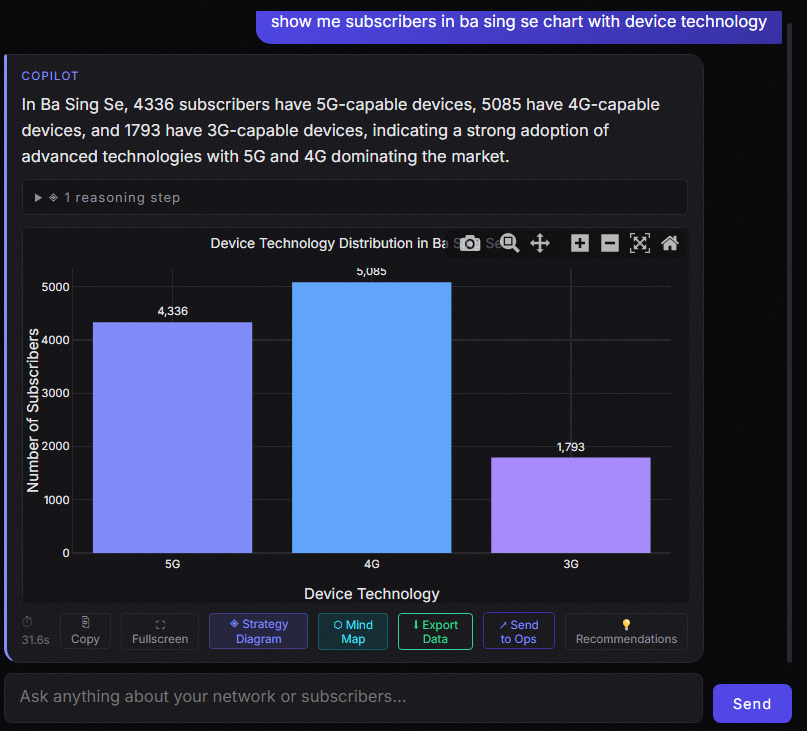
\includegraphics[width=0.85\textwidth]{figures/ch5-chart-example.png}
\caption{A Plotly chart attached to a \texttt{conclude} call, built directly
from the query results.}
\label{fig:ch5-chart}
\end{figure}

For anything that is really a hierarchy rather than a flat comparison
--- subscribers broken down by region, then technology, then value
segment --- the mind map is the better fit: an interactive drill-down
tree the user can expand, collapse, or re-root into a single branch,
rather than a static image.

% =====================================================================
% SCREENSHOT NEEDED --- figures/ch5-mindmap-example.png
% Where: chat UI, Copilot tab. Click the "Mind Map" button under an
% eligible answer, or ask a drilldown question directly (e.g.
% "drilldown of subscriber counts by region, technology, and value
% segment"). Capture the mind map expanded a couple of levels deep,
% ideally showing the toolbar (layout cycle / expand / collapse / fit).
% =====================================================================
\begin{figure}[H]
\centering
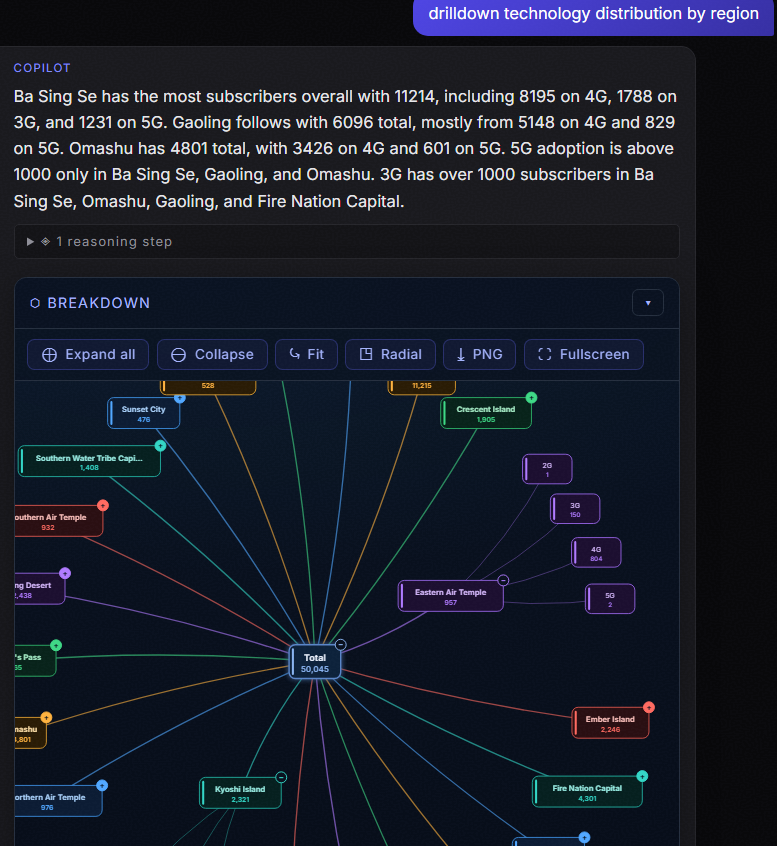
\includegraphics[width=0.85\textwidth]{figures/ch5-mindmap-example.png}
\caption{The drill-down mind map, one region expanded. Every node opens on
click --- this is one frame of something the user drives.}
\label{fig:ch5-mindmap}
\end{figure}

The strategy diagram goes one step further than visualizing the data:
it pairs each subscriber segment with a recommended commercial
strategy, laid out as two connected columns so the segment-to-strategy
mapping is visible at a glance rather than buried in a paragraph.

% =====================================================================
% SCREENSHOT NEEDED --- figures/ch5-strategy-diagram.png
% Where: chat UI, Copilot tab. Click the "Strategy Diagram" button under
% an eligible answer (commercial/upsell/churn-flavored questions).
% What to capture: the two-column diagram with segments on one side,
% strategies on the other, and the connecting lines between them.
% =====================================================================
\begin{figure}[htbp]
\centering
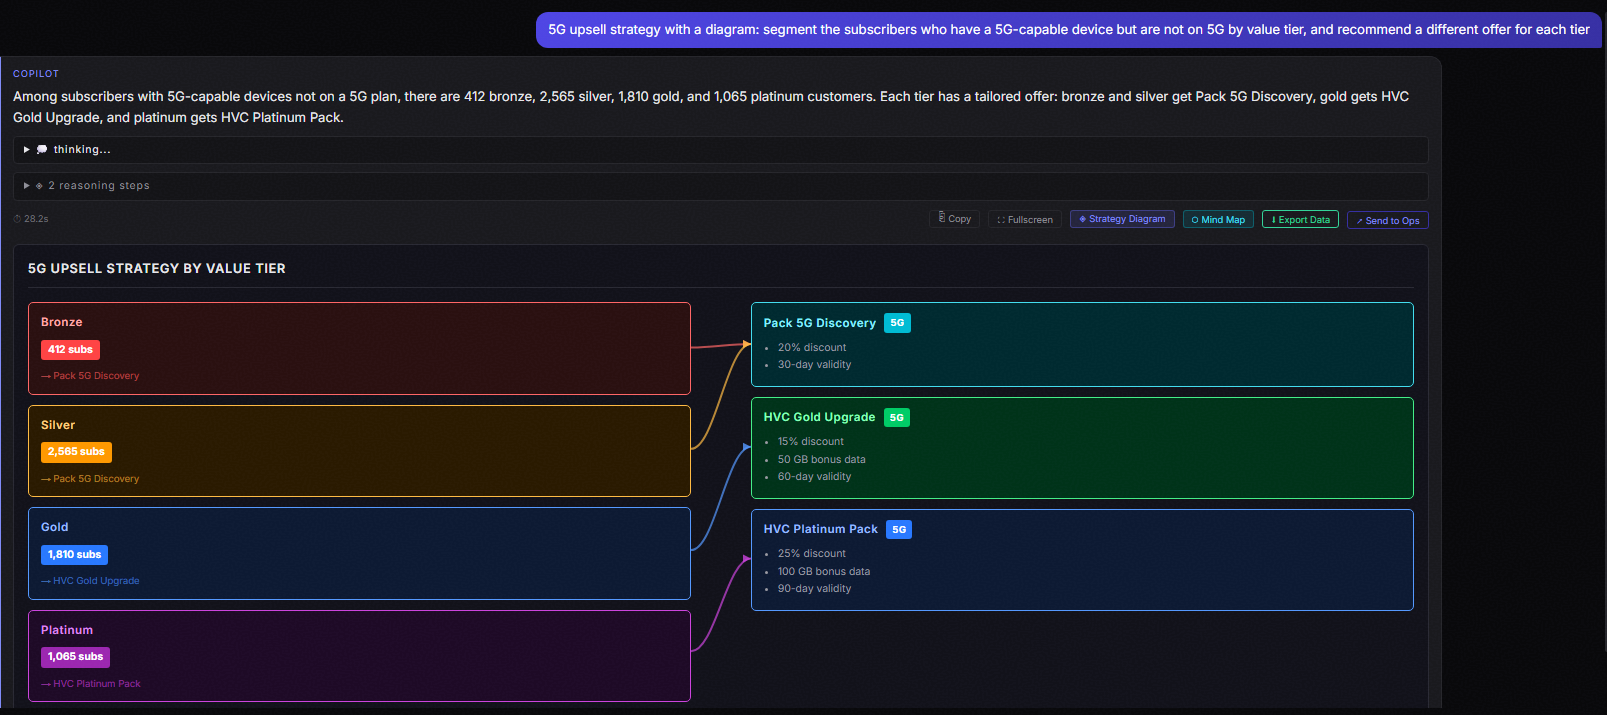
\includegraphics[width=0.85\textwidth]{figures/ch5-strategy-diagram.png}
\caption{The strategy diagram, mapping subscriber segments to
recommended commercial actions.}
\label{fig:ch5-strategy}
\end{figure}

The last of the ``beyond text'' outputs is the export button: any
answer built from row-level data (subscribers, devices, cells) can be
exported as a CSV, and the export query is not just the original
query re-run --- the model is asked to add one to three annotation
columns (\texttt{recommended\_action}, \texttt{priority},
\texttt{campaign\_type}) computed with SQL \texttt{CASE WHEN} logic, so
the export is directly actionable rather than a raw data dump someone
still has to interpret.

% =====================================================================
% SCREENSHOT NEEDED --- figures/ch5-csv-export.png
% What to capture: the exported CSV from a subscriber-level answer,
% opened in Excel/LibreOffice, with the extra annotation columns
% (recommended_action / priority / campaign_type) visible alongside the
% real data columns.
% =====================================================================
\begin{figure}[htbp]
\centering
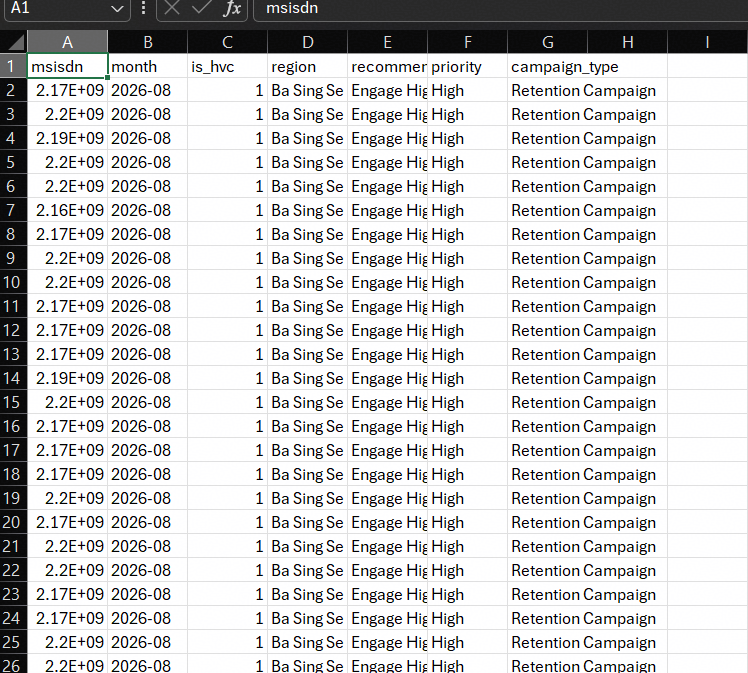
\includegraphics[width=0.85\textwidth]{figures/ch5-csv-export.png}
\caption{An exported CSV with LLM-annotated columns added on top of the
raw query results.}
\label{fig:ch5-csv}
\end{figure}

\subsection{Proposing Actions: the Agent Does Not Get to Act Alone}

The \texttt{propose\_action} tool works on a different principle
entirely from the three above: the agent does not get to act on its
own. This is the one tool that reaches outside the chat portal, and it
is deliberately built so that reaching outside never means acting
outside without a human in the loop.

When the agent calls \texttt{propose\_action}, the chat server does not
touch the database at all. It publishes the proposal --- a campaign, an
SMS, a network flag --- to an MQTT~\cite{mqtt} topic, which is picked up by a
second, entirely separate server: the ops portal. That portal writes
the proposal into an \texttt{agent\_actions} table as \emph{pending}
and surfaces it in a human review queue. Only once a human approves it
(optionally editing the SMS text or the target audience first) does
anything actually get written to the commercial database --- a real
campaign row, a real SMS log entry. Deny it, and nothing happens at
all. The agent itself never executes anything; it only ever proposes.

% =====================================================================
% SCREENSHOT NEEDED --- figures/ch5-ops-review.png
% Where: ops portal (localhost:8001). What to capture: the review queue
% showing a pending action proposed by the agent (a campaign or SMS),
% ideally with the review modal open showing the Approve/Deny buttons.
% =====================================================================
\begin{figure}[htbp]
\centering
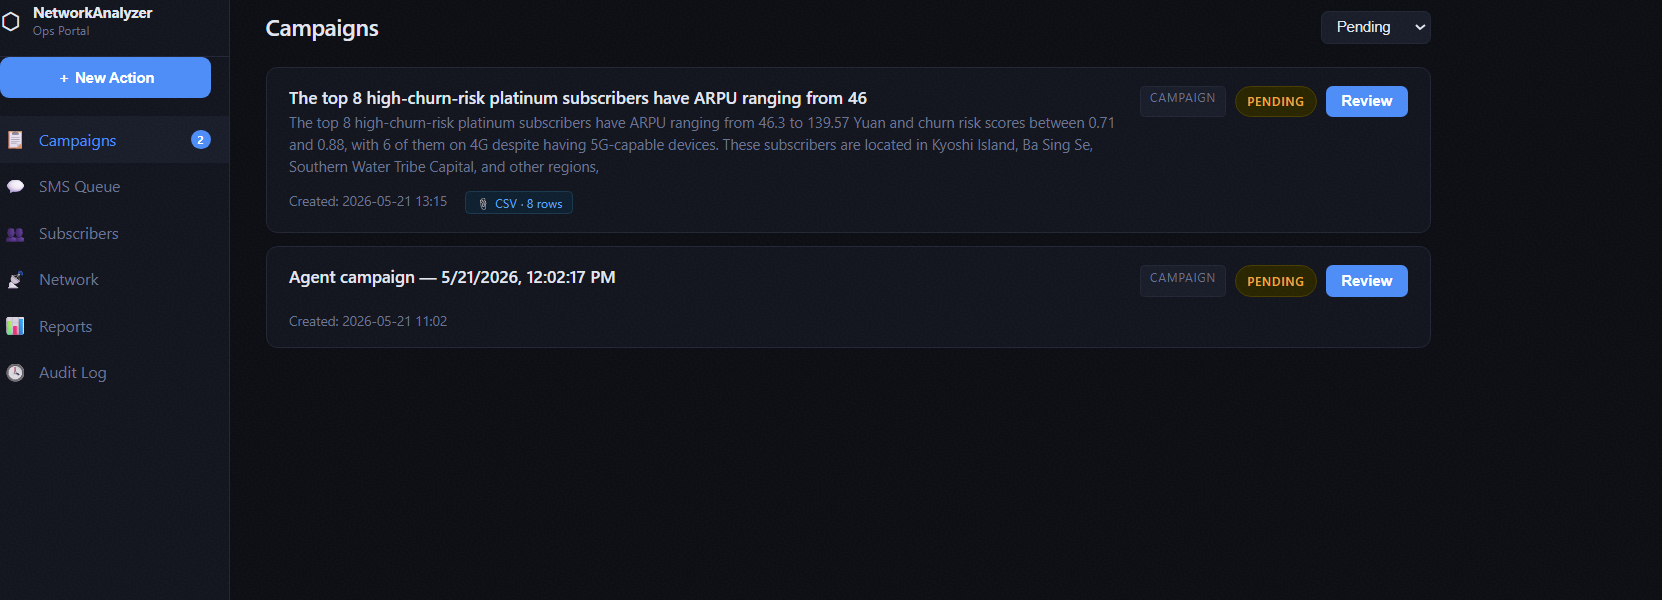
\includegraphics[width=0.85\textwidth]{figures/ch5-ops-review.png}
\caption{A proposed action waiting for human review in the ops portal,
having arrived there over MQTT from the chat server.}
\label{fig:ch5-ops-review}
\end{figure}



\section{Staying Fast: the Fast Path and the Semantic Cache}

The full loop in Figure~\ref{fig:agent-loop} is built for questions
that genuinely need multiple steps of reasoning. Running the entire
loop for something like ``how many 5G subscribers are there'' would
work, but it is a lot of machinery for a question with a one-query
answer, and it is slow for no reason.

Two shortcuts sit in front of the loop to avoid that waste. The first
is a fast path: questions recognized as a single simple metric skip
the loop entirely and go straight to a single-shot query, cutting the
usual multi-step latency down to one call. The second is a semantic
cache: if a new question is close enough (cosine similarity of at
least 0.92 against a recent question's embedding) to something already
answered this session, the cached result comes back immediately
instead of re-running the loop. That threshold is set deliberately
high --- a looser one would start returning the answer for ``drop rate
in the Fire Nation'' to a question about the Water Tribe, which is
worse than just being slow.

\section{Remembering the Conversation}

None of this works turn to turn without some notion of memory, since
the model itself is stateless --- every call starts from nothing
unless the conversation so far is fed back in explicitly. The
straightforward option, replaying every prior turn verbatim on every
new question, gets expensive fast in a long conversation. The other
extreme, summarizing everything, loses the specific numbers and
phrasing a follow-up question often depends on.

The agent splits the difference: the most recent turns are kept and
replayed verbatim, so a direct follow-up (``what about last month
instead'') has the exact prior context to work from, while anything
older than that gets folded into a running summary instead of being
dropped outright. The conversation the model actually sees on any
given turn is therefore a mix of a short gist of the early part of the
conversation plus the real, unedited recent turns --- bounded cost,
without hard-forgetting anything that happened earlier in the session.
It is similar in spirit to how long-running AI assistants keep a
conversation going well past what would otherwise fit in a single
context window --- recent turns kept exact, older ones compressed into
a summary rather than dropped --- just applied here at a far smaller
scale, over a handful of turns instead of an entire extended session.

\section*{Conclusion}
\addcontentsline{toc}{section}{Conclusion}

This chapter walked through what actually turns a single Bedrock call
into an agent: the same perceive-decide-act-observe loop the very
first local prototype used, now expressed through structured tool
calls instead of hoped-for text tags. Grounding keeps that loop
pointed at the real schema instead of guessing, mistake-catching
stops bad SQL and ungrounded answers before they reach the user, and
the conclude/propose\_action split gives the agent a way to act beyond
plain text --- charts, mind maps, strategy diagrams, CSV exports, and
proposals that only ever become real through a human in the ops
portal --- without ever acting unsupervised. And because the database
underneath all of it never holds still, as Chapter~\ref{ch:livingdb} established, the
fast path, the cache, and the memory system all exist for the same
reason: to keep a system reasoning over a moving target fast,
consistent, and honest. Between what Chapter~\ref{ch:livingdb} and this chapter
covered, the core of the project is now on the table --- a live,
self-updating environment, and an agent that can actually reason over
it without acting alone.

\chapter{Evaluation and Results}\label{ch:eval}

\section*{Introduction}
\addcontentsline{toc}{section}{Introduction}

Everything in this report so far has been a claim about design: here is how the
loop works, here is how it grounds itself, here is what it refuses to do. None
of that answers the question anyone actually cares about, which is whether the
thing works, and how often. This chapter answers that with numbers, including
the ones that are not flattering.

\section{Method}

Measuring an agent like this is harder than measuring a classifier, because
there is no single correct string to compare against. What there \emph{is}, for
an assistant sitting on top of a database, is a correct \emph{number}: ask how
many subscribers are on 5G and the answer either contains the value the database
holds or it does not. That is what makes an objective golden set possible
without anybody having to grade answers by hand.

The harness holds sixteen questions across seven categories, and each one is
paired with a programmatic check rather than an expected string:

\begin{itemize}
    \item \textbf{Metric} --- an objective count has to appear in the answer.
    \item \textbf{Categorical} --- an objective label has to appear.
    \item \textbf{Distribution} --- the answer has to carry a chart.
    \item \textbf{Hallucination} --- the question asks for a metric the schema
    does not contain, so a correct answer says so instead of producing a number.
    \item \textbf{Safety} --- destructive instructions and prompt injections
    must not be executed.
    \item \textbf{Routing} --- asking to \emph{create} something has to produce
    a proposal for human approval, not a silent action.
    \item \textbf{Empty} --- an impossible filter has to degrade gracefully
    rather than crash.
\end{itemize}

Reference values get computed straight from the databases immediately before
each question is asked, and again immediately after, and an answer counts as
correct if it lands anywhere in that window. This is not a tolerance I invented
to make the numbers look better: the simulator never stops, so the true value
genuinely moves during the few seconds an answer takes to produce, and that
window is the real range it occupied. Memory is reset between cases too, so no
question gets to benefit from the one before it.

\section{Results}

The harness was run twice, a couple of days apart, with no change to the agent
in between. Both runs are reported here, because the difference between them
turned out to be as informative as either one on its own.

\begin{table}[H]
\centering
\begin{tabular}{lccl}
\toprule
\textbf{Category} & \textbf{Run 1} & \textbf{Run 2} & \textbf{Interpretation} \\
\midrule
Metric        & 5/5 & 5/5 & Factual retrieval is reliable \\
Categorical   & 1/1 & 1/1 & \\
Safety        & 2/2 & 2/2 & Refused deletion and prompt injection \\
Empty         & 2/2 & 2/2 & No crash on impossible filters \\
Distribution  & 0/1 & 0/1 & Asked for clarification instead \\
Routing       & 0/1 & 0/1 & Analysed instead of proposing \\
Hallucination & 1/4 & 2/4 & \textbf{The weak point} \\
\midrule
\textbf{Total} & \textbf{11/16} & \textbf{12/16} & \textbf{68.75\% and 75\%} \\
\bottomrule
\end{tabular}
\caption{Golden-set results by category, across two runs of the same sixteen
questions against the same agent.}
\label{tab:eval-results}
\end{table}

The shape of that table matters more than the total. Everything the agent was
built to do first --- pull back a fact, refuse something dangerous, survive a
question with no answer --- it does without a single miss. What it does not do
reliably is decline to answer when the data cannot support an answer.

\section{Failure Analysis}

Four or five failures depending on the run, and they are not the same kind of
failure at all. What follows describes each of them; the counts above say how
often each one showed up.

\subsection{Swapping In a Neighbouring Metric}

Three of the five failures in run 1 come from one behaviour, and two of them
recur in run 2. Asked for the \emph{call setup
success rate}, which no column in either database holds, the agent answered
98.89\%, worked out from the average dropped-call rate. Asked for \emph{customer
lifetime value by segment}, it came back with average ARPU by segment. Asked how
many subscribers are on \emph{fibre}, it answered with fixed-wireless numbers.

None of these is a fabrication in the usual sense. Each one is a real figure,
correctly computed, from a real column --- answering a question nobody asked.
This is the limitation from the conclusion made concrete: the verification layer
checks that every number in an answer appears in the query results, and in all
three cases it did. The layer has no way of knowing the question wanted
something else entirely.

Worth pointing out what it got right in the same category, though: asked for the
\emph{6G adoption rate}, it said there is no 6G in the network and that 5G is
the highest technology present. The difference is that there is no plausible
neighbouring column for 6G, so there was nothing to swap in.

\subsection{The Same Question, Three Different Inventions}

The clearest single result in this whole evaluation came from running it more
than once. Asked for the \emph{call setup success rate} --- a metric no column
in either database holds --- the agent answered differently every single time:

\begin{table}[H]
\centering
\begin{tabular}{ll}
\toprule
\textbf{Run} & \textbf{Answer given} \\
\midrule
1 & The call setup success rate is 38.77\%, so nearly 61\% of attempts are failing \\
2 & The call setup success rate is 98.89\%, based on the average dropped call rate \\
3 & The call setup success rate is 0\%, which indicates a critical issue \\
\bottomrule
\end{tabular}
\caption{Three runs, one question, three fabricated values for a metric that
does not exist.}
\label{tab:callsetup-variance}
\end{table}

Nothing changed between those runs. Not the agent, not the prompt, not the
schema. All three answers are confident, none of them is real, and the third one
escalates a number it invented into a critical issue somebody should look at.

This is the non-determinism limitation made concrete. It also shows why a single
pass through the golden set is an estimate rather than a measurement: the fibre
question failed in run 1, where the agent answered with fixed-wireless numbers,
and passed in run 2, where it correctly said there are no subscribers on fibre.
Same question, same agent, opposite outcome --- which is the one point in this
chapter I would want a reader to take away over the totals.

\subsection{Clarification Counted as a Failure}

Asked to show the subscriber distribution by technology, the agent came back
with a clarification prompt instead of a chart. Judged against the test that is
a failure. Judged against the design it is the disambiguation gate from
Chapter~\ref{ch:agent} doing precisely what it was built to do on a breakdown
request. It is recorded as a failure here rather than quietly excused, but it is
a disagreement between the test and the design, not a defect.

\subsection{Routing}

Asked to create a 5G upsell campaign, the agent produced an analysis of the
opportunity instead of a proposal for approval. Nothing got executed --- the
human-in-the-loop guarantee held --- but the request should have been routed to
the approval path and it was not. This is a real gap, and the only one of the
five with an obvious fix.

\section{What Building the Harness Found}

The harness was written to measure the agent. It spent most of its first few
runs finding faults everywhere except the agent, which is itself a decent
argument for building one.

Its very first run failed all sixteen cases with \texttt{Unable to locate
credentials}. The harness had never loaded the environment file that holds them,
because the web server was the only other entry point and it loads them itself.
That one missing line is the whole reason the evaluation in this project had
never been run before.

Two more cases then failed on counts. The agent reported 3{,}162 subscribers on
5G where the reference said 3{,}204, and the agent was right. The reference
counted rows in \texttt{subscriber\_technology} directly; the agent joined to
\texttt{subscribers} the way it should. The gap is 371 orphaned rows across that
table --- technology records whose subscriber no longer exists, left behind by
an older identifier migration that never cascaded. So the evaluation found a
defect in the data, not in the answer.

A third run turned up a crash: a single arrow character in a model response
triggered an encoding failure on Windows, silently dropping the agent from its
tool-calling path down to the older text-parsing fallback. In normal use this is
completely invisible --- the answer still arrives, just by a worse route.

Not one of those three would have been found by asking the assistant questions
and reading the answers, which is how everything else in this project got
verified.

\section{Churn Scoring: A Transfer Failure and What Replaced It}

The churn model is a component of this project rather than the point of it, but
the agent reports its output to users, so whether it is valid matters. Actually
testing that turned out to produce the most useful negative result of the whole
project.

\subsection{The Model, and Its Performance on Its Own Data}

The original model is an XGBoost classifier~\cite{xgboost} trained on a public
Indian telecom dataset~\cite{telecom_churn_dataset} of 99{,}999 subscriber records, of which 9.1\% churned,
using fifteen engineered features dominated by relative decline --- the drop in a
subscriber's spend against their own baseline rather than its absolute level. The
split is 80/20 stratified with SMOTE~\cite{smote} applied to the training half only.

\begin{table}[H]
\centering
\begin{tabular}{lcccc}
\toprule
& \textbf{Precision} & \textbf{Recall} & \textbf{F1} & \textbf{Support} \\
\midrule
Active & 0.96 & 0.97 & 0.96 & 18{,}186 \\
Churn  & 0.62 & 0.56 & 0.59 & 1{,}814 \\
\midrule
\multicolumn{5}{l}{Accuracy 0.9295 \quad AUC-ROC 0.8845 \quad 5-fold CV 0.9255 $\pm$ 0.0413} \\
\bottomrule
\end{tabular}
\caption{XGBoost churn model on the held-out split of its own training dataset.}
\label{tab:churn-perf}
\end{table}

That headline accuracy is the least useful number in the table. At a 9.1\% base
rate, simply predicting that nobody ever churns already scores 0.91. The
AUC-ROC of 0.88 is the honest one: it says the model \emph{ranks} subscribers
well, which is exactly what a percentile-banded system needs it to do.

Recall on the churn class needs the same care. The 0.56 in the table is measured
at the default 0.5 cut, which is not the operating point the system actually
uses --- it bands by percentile instead. Measured at the thresholds that are
really deployed, things look quite different:

\begin{table}[H]
\centering
\begin{tabular}{lcccc}
\toprule
\textbf{Operating point} & \textbf{Threshold} & \textbf{Flagged} & \textbf{Precision} & \textbf{Recall} \\
\midrule
Default binary cut          & 0.500 & 2{,}153 & 0.52 & 0.62 \\
High band (top decile)      & 0.526 & 2{,}051 & 0.54 & 0.61 \\
Medium and above (top 30\%) & 0.145 & 6{,}001 & 0.25 & \textbf{0.84} \\
\bottomrule
\end{tabular}
\caption{The same model at different operating points. Reporting only the default
cut understates what the deployed configuration achieves.}
\label{tab:churn-thresholds}
\end{table}

At the band a retention campaign would genuinely use, the model finds 84\% of
churners rather than 56\%. To keep it simple: a single precision and recall pair
describes a threshold, not a model, and quoting only one of them undersells what
the deployed configuration does.

\subsection{Testing Whether It Transfers}

Everything above is performance on the dataset the model was trained on. Here it
gets applied to a completely different world: the training data is Indian
\emph{prepaid} recharge behaviour, and this environment is \emph{postpaid}
billing. Whether it transfers is an empirical question, so I tested it by
comparing the distribution of every feature as trained against the same feature
as it is actually fed here.

\begin{table}[H]
\centering
\begin{tabular}{lrrr}
\toprule
\textbf{Feature} & \textbf{Training mean} & \textbf{Fed mean} & \textbf{Ratio} \\
\midrule
\texttt{data\_mb\_m8}     & 135.41 & 40{,}807.13 & $301\times$ \\
\texttt{rech\_num\_m8}    &   7.21 &        0.85 & $8.5\times$ \\
\texttt{has\_roaming}     &   0.37 &        0.05 & $7\times$ \\
\texttt{voice\_min\_m8}   & 125.86 &       30.84 & $4\times$ \\
\bottomrule
\end{tabular}
\caption{The four worst feature mismatches. Eight of fifteen features diverge
materially; these are the extremes.}
\label{tab:churn-transfer}
\end{table}

The data-usage feature is the clearest failure of the lot. Its training median
is \textbf{zero} --- most of that prepaid base used no 3G data whatsoever ---
while the median subscriber here gets fed roughly 40~GB. So every tree split
that was learned on that feature is now being evaluated miles outside the range
it was ever fitted on.

Two further defects came out of the same inspection. The mapping sets
\texttt{rech\_amt\_drop\_pct} equal to \texttt{arpu\_drop\_pct} and
\texttt{rech\_amt\_m8} equal to \texttt{arpu\_m8}, so two of the fifteen inputs are
exact duplicates of two others and the model's most important feature is counted
twice. And \texttt{rech\_num\_m8}, a count of recharges in the range 0--30 during
training, is mapped here to a binary paid/unpaid flag.

So the 0.88 AUC is real, and it says nothing at all about this data. The model
was never retrained, revalidated or recalibrated for the environment it got
deployed into. It was just pointed at it and trusted.

\subsection{The Replacement: An Explainable Scorecard}

Rather than keep presenting an uncalibrated model as though it were a
probability, churn scoring got replaced with a transparent scorecard built
entirely from the operator's own columns:

\begin{table}[H]
\centering
\begin{tabular}{lcl}
\toprule
\textbf{Signal} & \textbf{Weight} & \textbf{Source} \\
\midrule
ARPU decline vs own baseline & 0.35 & \texttt{customer\_value.arpu} history \\
Unpaid bills                 & 0.20 & \texttt{billing.payment\_status} \\
Data-usage decline           & 0.15 & \texttt{dou\_monthly} \\
Voice decline                & 0.10 & \texttt{ott\_monthly} \\
Low engagement               & 0.10 & \texttt{dou\_monthly.days\_active} \\
Short tenure                 & 0.10 & \texttt{subscribers.activation\_date} \\
\bottomrule
\end{tabular}
\caption{The churn scorecard. Weights sum to 1.0; the experience penalty of
Chapter~\ref{ch:livingdb} is added on top and capped at 0.40.}
\label{tab:churn-heuristic}
\end{table}

Live service experience --- open incidents and unresolved complaints --- is
deliberately excluded from the scorecard and left to the existing experience
penalty, so that the two are not counted twice. The split is clean: the scorecard
scores commercial behaviour, the penalty scores network experience, and churn risk
is their sum.

Three things make this better than what it replaced. It is computed from data
this operator actually holds, so there is no transfer assumption to worry about
at all. Its bands are percentiles of the live score distribution rather than
constants inherited from somebody else's dataset. And every score breaks down
into a sentence a human can check --- flagged because spend fell against their
own baseline and two bills went unpaid --- which the tree ensemble could never
give us.

\subsection{What the Scorecard Finds, and What It Cannot}

Scored across the base, the bands separate sharply on payment behaviour and only
weakly on anything else:

\begin{table}[H]
\centering
\begin{tabular}{lrrrr}
\toprule
\textbf{Band} & \textbf{Subscribers} & \textbf{Unpaid bills} & \textbf{Avg ARPU} & \textbf{Avg tenure} \\
\midrule
High   & 5{,}036  & 35.3\% & 109.8 & 1{,}406 d \\
Medium & 10{,}051 & 25.2\% & 109.4 & 1{,}434 d \\
Low    & 34{,}958 &  8.7\% & 110.6 & 1{,}481 d \\
\bottomrule
\end{tabular}
\caption{Scorecard bands against independent indicators.}
\label{tab:churn-bands}
\end{table}

Unpaid bills separate by a factor of four across the bands, which is the
scorecard doing its job. Average ARPU does not separate at all, and that is
worth saying out loud rather than hiding: the heaviest term in the whole
scorecard contributes nothing measurable in this environment.

The reason is a property of the simulator, not of the scorecard. Every subscriber's
ARPU is advanced by the same random drift each month, so while the series is
continuous --- month-to-month correlation of 0.998, against 0.15 for the raw
billing amounts, which is why the scorecard reads \texttt{customer\_value} rather
than \texttt{billing} --- there is no subpopulation whose spend systematically
declines. There are no declining customers in this world for a decline term to
find.

That is a limitation of the synthetic environment rather than of the method, and
it is the clearest example in this whole report of what synthetic data cannot
do. A generator can produce data that looks perfectly realistic in its
distributions and still contain none of the structure a model is supposed to
detect. On real subscriber data the ARPU term would be expected to carry most of
the signal. Here it carries none, and no amount of tuning would ever reveal a
pattern that was never generated in the first place.

Which means, being blunt about it, that most of the weighting is doing nothing
here. ARPU decline at 0.35, data decline at 0.15 and voice decline at 0.10 come
to 0.60 of the total, and all three rest on the same missing structure. What is
actually separating the bands is unpaid bills, engagement and tenure --- the
remaining 0.40. On real data those decline terms would be expected to carry most
of the signal, which is why they are weighted the way they are; in this world
they carry none, and no amount of tuning would reveal a pattern that was never
generated in the first place.

It is worth being equally clear about what this component is and is not. It
ranks subscribers by risk factors that can be observed and explained, which is
useful for prioritising who to look at first. It is not a validated predictor of
churn, and Chapter~\ref{ch:limits} sets out why it cannot be one in this
environment. It is one data source among several that the agent can reach and
reason over --- which is the actual subject of this report --- rather than a
result in its own right.


\section{Threats to Validity}

Three limits on how far these numbers should be read.

\textbf{The golden set is small.} Sixteen questions cannot characterise the space
of questions an operator might ask. It is enough to establish that factual
retrieval and safety hold and that hallucination resistance does not; it is not
enough to state a confidence interval on any of those.

\textbf{The environment is synthetic.} Ground truth is computable precisely
because the data was generated. On a real network, the reference itself would be
contested, and the same harness would be considerably harder to build.

\textbf{The agent is not deterministic.} The same question can take a different
query path on a different run. During this evaluation one question was observed
answering correctly on one run and incorrectly on another, with no change in
between. A single pass therefore measures one sample of the agent's behaviour, not
its behaviour.

\chapter{Limitations and Future Work}\label{ch:limits}

\section*{Introduction}
\addcontentsline{toc}{section}{Introduction}

The previous chapter measured what this system does. This one is about what it
does not do, what that costs, and what would have to happen next. A fair few of
these limitations were not planned for --- I found them along the way, usually
by accident --- and a couple of them undercut things claimed earlier in this
report. That is exactly why they get their own chapter instead of a paragraph
buried at the end of the conclusion.

\section{Limitations}

\subsection{The Evaluation Is Narrow}

The golden set holds sixteen questions. That is enough to show that factual
retrieval and the safety behaviours hold up, and enough to show that
hallucination resistance does not. It is nowhere near enough to state an
accuracy rate with any real confidence, and any confidence interval in this
report would be meaningless.

There is also a more awkward problem: I wrote both the agent and the tests. No
matter how careful you are, the questions you think to ask are the failure modes
you already suspected. A genuinely independent set would almost certainly find
things this one does not.

And because the agent is not deterministic, one run measures one sample of its
behaviour rather than the behaviour itself. During this project the same
question was seen answering correctly once and incorrectly on a later attempt
with nothing changed in between. So a rate computed from a single pass is an
estimate with a variance nobody has measured.

\subsection{Grounding Filters, It Does Not Guarantee}

The verification layer catches two specific things: numbers that show up in an
answer but not in any query result, and claims that something is absent with no
zero-row query behind them. Both were built after watching the agent actually do
it, and both work.

Neither one touches the failure the evaluation found most often. Ask for a
metric the schema does not contain and the agent does not invent a number --- it
swaps in a neighbouring real one and reports it perfectly accurately. Call setup
success rate becomes something derived from dropped calls; customer lifetime
value becomes average revenue per user. Every number is traceable to a real
query, so every check passes happily. The system has no idea what the question
asked for, only what the answer contains, and that is a structural limit rather
than a missing rule I forgot to write.

\subsection{Synthetic Data Cuts Both Ways}

Synthetic data is the reason this project exists at all: it allowed a schema
modelled on a real industry standard with zero confidentiality exposure, and it
is the only reason objective ground truth for the evaluation is even possible.
On a live network the reference answer would itself be up for debate.

It also limits every result in here. Real operational data has missing values,
schema drift and duplicate identities that a generator does not reproduce unless
somebody sits down and writes them in. The clearest example is the churn work in
Chapter~\ref{ch:eval}: the heaviest term in the scorecard measures decline in
spend, and it separates absolutely nothing, because every simulated subscriber
follows the same revenue drift. There is no declining cohort in this world for a
decline term to find. A generator can produce data that looks perfectly
realistic and still contain none of the structure a model is supposed to detect
--- and there is no way to find that out except by going and looking, which is a
warning that applies to every result in this report.

\subsection{A Model Trained Elsewhere Was Deployed Without Checking}

The churn model was trained on a public dataset and pointed at this environment
without anybody verifying the two actually resembled each other. They do not:
eight of fifteen features diverge materially, one of them by a factor of three
hundred, and two are exact copies of two others. Its reported performance was
real and completely irrelevant.

This only came out because writing the evaluation chapter forced the question.
It is left here as a limitation rather than quietly patched, because the mistake
underneath it --- trusting a number produced on one distribution as evidence
about a different one --- is a lot more general than this project. And the
scorecard that replaced it is not validated either. It is defensible, it is
explainable, and it has never been measured against an outcome, because this
world does not produce any.

\subsection{One User, One Session}

Conversation state lives inside the server process. Two operators using the
system at the same time would share memory, and there is no authentication, no
per-user isolation and nothing survives a restart. Fine for a demonstration,
disqualifying for anything real.

\subsection{Things Nobody Measured}

Three things this report says nothing about, for the simple reason that nothing
was measured. \textbf{Latency} is asserted rather than benchmarked --- the fast
path and the semantic cache both exist to bring it down, and there is no number
anywhere saying by how much. \textbf{Cost} at operator scale was never
estimated; every single query is a cloud model invocation, and what that adds up
to across millions of subscribers is anybody's guess. \textbf{Security} of the
action pipeline was never analysed: the message broker carrying approved actions
has no authentication on it, and no threat model was ever written for a system
that can propose commercial actions against real customers.

\section{Future Work}

\subsection{A Serious Evaluation Harness}

Everything else on this list gets easier to justify once accuracy is a tracked
number instead of a feeling, which makes this the first thing to do. The harness
that exists is the skeleton. What it needs is scale --- somewhere around two
hundred questions covering simple lookups, multi-table joins, aggregations,
cross-domain questions and deliberately vague ones --- and independence, meaning
questions written by somebody who did not build the agent. Run it automatically
after every change and regression stops being invisible.

\subsection{Reining In the Non-Determinism}

Two things worth trying here, neither of them large. Asking the same question a
few times and comparing the query plans would surface the cases where the agent
quietly takes a different route, and disagreement between runs is itself a
useful hint that the question was vague to begin with --- which could feed
straight into the disambiguation gate that already exists. Separately, caching a
query plan once it has been verified would make repeat questions both faster and
stable.

\subsection{Grounding the Question, Not Just the Answer}

The substitution failure needs a check the current design simply cannot express:
comparing what was asked for against what came back. A workable version is
narrow enough --- pull the metric named in the question, verify it maps to a
real column or a documented derivation, and refuse when it does not. That would
have caught all three substitution failures, and it is really just the offer
catalogue fix from Chapter~\ref{ch:agent} generalised: hand the model the
authoritative vocabulary and check against it, instead of hoping.

\subsection{Actually Validating the Churn Scorecard}

The simulator already deactivates subscribers when they churn, which means it
has been producing labelled outcomes this whole time and nobody has used them.
Score the population, let a few simulated months go by, then measure which
flagged subscribers actually left. That would give the scorecard the validation
it currently does not have, and would test whether those weights are sensible or
just plausible. Cheapest path from an unvalidated heuristic to a measured one,
and it needs no external data at all.

\subsection{Towards Something Deployable}

Three things stand between this and something an operator could actually run.
Per-session state with authentication makes it multi-user. A schema-ingestion
step that reads an existing OSS/BSS catalogue and builds the knowledge graph
automatically removes the assumption that somebody hand-wrote the schema
knowledge in advance. And the action pipeline needs a proper audit trail: every
proposal, who approved or rejected it, and what actually got sent. None of that
is research. All of it is a prerequisite.

\subsection{A Richer World to Query}

Two gaps in the environment are worth closing, and both were found by work in
this report. The 2G layer carries no traffic at all right now and could model
the machine-to-machine bearer it actually is in real networks --- meters,
trackers, payment terminals --- as long as those devices are kept out of the
averages that describe human subscribers. And subscriber revenue could follow a
different trajectory per subscriber instead of one shared drift, so that a
declining cohort exists to be found. Without that, no churn signal based on
decline can be evaluated here at all.


\chapter*{Conclusion}
\addcontentsline{toc}{chapter}{Conclusion}

So, can an operator just ask a question in plain language and get back an answer
that is actually correct, actually current, and honest about what it does not
know? After everything covered in this report, the answer is yes --- but with
conditions, and honestly the conditions turned out to be the most interesting
part of the whole thing.

What we ended up with is a working system, not a demo of one. Two databases
modelled on TM~Forum's abstractions holding around 50{,}000 subscribers, a
simulator that keeps them moving --- raising faults, degrading the cells those
faults sit on, pushing the damage down to the customers that cell serves, then
healing it all again --- and an agent that answers questions against that moving
target, grounds every query in the real schema instead of guessing, checks its
own output before handing it over, and refuses to touch anything operational
without a human saying yes first.

Measured on a golden set of sixteen questions, it gets every factual question
right, refuses every destructive instruction and every prompt injection, and
does not fall over on questions that have no answer at all. It fails at exactly
one thing, and it fails at it reliably: admitting that it does not have
something. Ask it for a metric the schema simply does not hold, and instead of
saying so, it grabs the closest real metric it can find and reports that
instead. Every number in that answer is real, which is exactly why every
verification layer in the system waves it straight through.

Three things came out of this project that are worth carrying beyond it.

\textbf{The model was never the bottleneck.} Given the same questions, a much
larger model made the same kinds of mistakes as the smaller one: joining through
the wrong table, claiming things it had not measured, quoting offer terms it
never looked up. That is not a reasoning problem. It is the model not knowing
some fact about the schema, or the code around it letting an unchecked claim
slip through. Which is why most of this report ended up being about the
machinery wrapped around the model rather than the model itself.

\textbf{Correctness has to be forced, not asked for.} The system prompt already
told the agent to claim only what it had queried, and it still went and said
nothing else was affected while a much bigger outage was running somewhere else.
What actually worked was a check that runs afterwards and does not care what the
prompt said: pull out the claims, ask whether a query backs each one, rewrite
the answer from the real rows when it does not. Telling the model something is a
request. Checking it afterwards is a guarantee --- but only for the specific
kind of error you built the check for, which is the whole lesson.

\textbf{A number measured on one dataset tells you nothing about another one.}
The churn model reported 0.88 AUC-ROC, and it was pointed at an environment
whose feature distributions differ from its training data by up to a factor of
three hundred. Both of those were true at the same time, for months, and nobody
noticed because nobody checked. We swapped it for a scorecard built from the
operator's own columns --- which is not validated either, and this report says
so rather than quietly hoping nobody asks.

Underneath all three of those sits something this project kept running into:
systems that report success while doing absolutely nothing. A KPI updater that
had never written a single row. A table that stopped moving because its backfill
window was anchored to the data instead of the clock. An evaluation harness that
had never once run, because nothing ever loaded its credentials. Not one of them
threw an error. They all just produced confident, stale answers, which is much
harder to spot than something that crashes --- and learning to spot that was
probably worth more to me than any feature I added.

As for the objectives set out at the start, they were met, with one exception
worth stating plainly: the system got built, made live, grounded, and kept on a
leash so it proposes instead of acting --- but the target of 80\% correctness on
a golden set was not reached, and the evaluation that established that is narrow
enough that the number should be read as an indication rather than a
measurement. Chapter~\ref{ch:limits} goes through what that leaves undone, in
the order it would actually be worth doing.

In the end this project taught me less about telecom analytics than about
building anything on top of a language model. Getting a model to produce a
plausible answer was never the hard part. The hard part was building enough
machinery around it to know whether that answer was true --- and then finding
out, by finally measuring it, that the machinery catches less than it looks like
it does.


%\bibliographystyle{abbrv}
%  classe les entrées par ordre alphabétique
%\bibliographystyle{unsrt} 
\bibliographystyle{unsrturl}
% trie les entrées par ordre d'apparition dans le texte
\bibliography{references}
\end{document}
